\chapter{Data Link Layer - Medium Access Control and Error Control}

\subsection{Coordinated Medium Access}

\noindent
\textbf{Tại sao cần điều phối (coordination)?}
\medskip

\noindent
Khi có nhiều card mạng (network interface card - NIC) cùng kết nối vào một đường truyền chung $\rightarrow$ việc truy cập cần phải được điều phối (need to be coordinated).

$\Rightarrow$ Nếu không có sự điều phối $\rightarrow$ collision sẽ xảy ra khi các thiết bị truyền dữ liệu cùng một lúc.
\medskip

\noindent
$\rightarrow$ Có 2 nhóm phương pháp điều phối.
\medskip

\noindent
\textbf{Contention-based Protocols (giao thức cạnh tranh):}

\begin{itemize}
    \item \textbf{Cơ chế:} các thiết bị tham gia phải cạnh tranh (compete) để truy cập vào đường truyền.
    \item \textbf{Đặc điểm:} \begin{itemize}
        \item Xử lý xung đột (collision handled) $\rightarrow$ do có nhiều thiết bị có thể gửi cùng lúc $\rightarrow$ xung đột là điều chắc chắn xảy ra $\Rightarrow$ protocol phải có cách xử lý chúng.
        \item Non-deterministic (không xác định trước được) $\rightarrow$ không thể biết trước ai sẽ gửi.
    \end{itemize}
    \item \textbf{Hiệu suất:} hoạt động tốt khi lưu lượng mạng thấp đến trung bình, và lưu lượng có tính chất đột biến (bursty).
    \item \textbf{Ví dụ:} ALOHA, CSMA/CA (tránh xung đột bằng cách nghe trước khi gửi - Carrier Sense Multiple Access with Collision Avoidance), MACA (Multiple Access with Collision Avoidance).
\end{itemize}
\medskip

\pagebreak

\noindent
\textbf{Contention-free Protocols (giao thức không cạnh tranh):}

\begin{itemize}
    \item \textbf{Cơ chế:} quyền truy cập đường truyền được phân bổ trước (allocated in advance).
    \item \textbf{Đặc điểm:} \begin{itemize}
        \item Tránh xung đột hoàn toàn (collision avoided) $\rightarrow$ collision không bao giờ xảy ra vì đã được plan trước.
        \item Deterministic (xác định trước được) $\rightarrow$ biết rõ ai sẽ gửi và gửi khi nào.
    \end{itemize}
    \item \textbf{Hiệu suất:} hoạt động tốt khi lưu lượng mạng cao (high utilization) $\rightarrow$ đảm bảo tính công bằng (guarantee fair use) về dung lượng mạng cho các thiết bị.
    \item \textbf{Ví dụ:} Token Passing, TDMA (phân chia theo thời gian - Time Division Multiple Access), FDMA (phân chia theo tần số - Frequency Division Multiple Access), CDMA (phân chia theo mã - Code Division Multiple Access).
\end{itemize}
\medskip

\section{Contention-based}

\subsection{ALOHA}

\subsubsection{ALOHA}

\noindent
ALOHA $\rightarrow$ \textbf{A}dditive \textbf{L}inks \textbf{O}n-line \textbf{H}awaii \textbf{A}rea $\rightarrow$ giao thức được phát triển tại Đại học Hawaii vào những năm 1970 để kết nối các trạm từ xa qua sóng vô tuyến.
\medskip

\noindent
\textbf{Pure ALOHA} $\rightarrow$ đây là phiên bản sơ khai và đơn giản nhất.
\medskip

\begin{figure}[h]
    \centering
    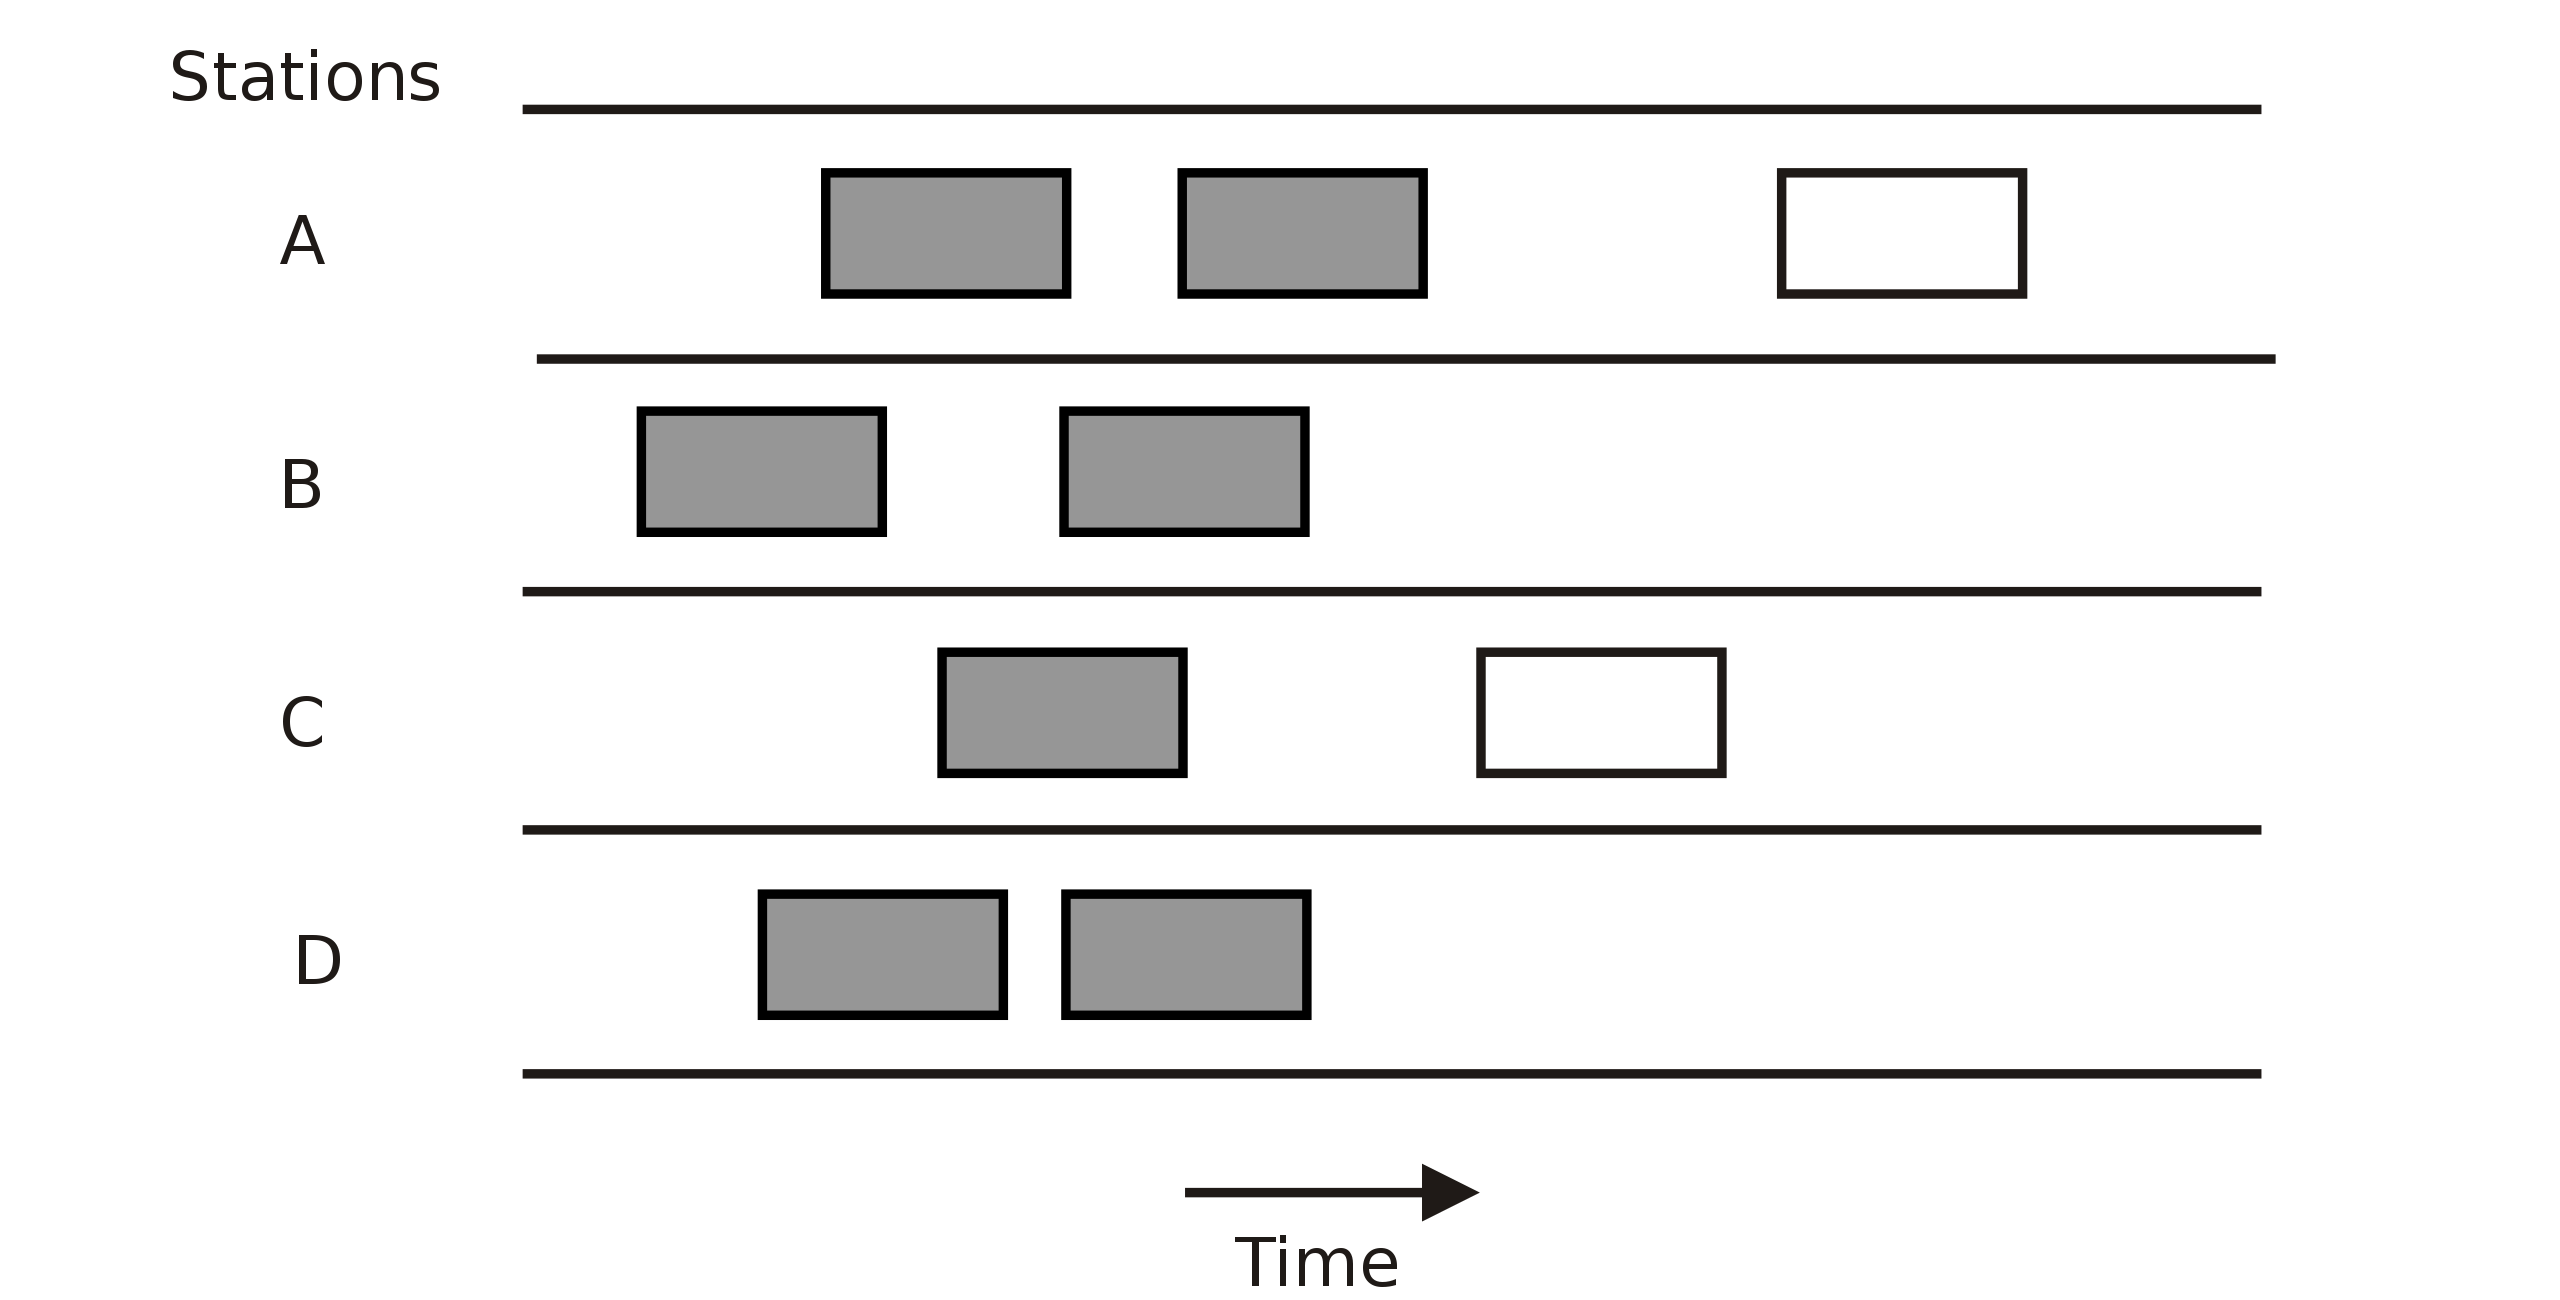
\includegraphics[width=0.6\textwidth]{assets/chap_4/aloha.png}
\end{figure}
\medskip

\begin{itemize}
    \item \textbf{Nguyên lý hoạt động:} không có kiểm soát trung tâm hay sự phối hợp nào giữa các trạm $\rightarrow$ các trạm có thể bắt đầu gửi dữ liệu bất cứ khi nào chúng muốn.
    \item \textbf{Vấn đề:} do ai cũng có thể nói bất cứ lúc nào $\rightarrow$ collision dễ xảy ra $\Rightarrow$ nếu 2 gói tin chồng lên nhau, dù chỉ một chút $\rightarrow$ cả 2 đều bị hỏng.
    \item \textbf{Đặc điểm:} \begin{itemize}
        \item Collision có thể xảy ra \textit{(như nãy nói trên)}.
        \item Không có tính công bằng (no fairness).
    \end{itemize}
\end{itemize}
\medskip

\noindent
$\Rightarrow$ Phương pháp rất đơn giản, không yêu cầu thêm gì.
\medskip

\subsubsection{Slotted ALOHA}

\noindent
Slotted ALOHA $\rightarrow$ ALOHA phân khe $\Rightarrow$ đây là phiên bản cải tiến của pure ALOHA để giảm thiểu collision.
\medskip

\begin{figure}[h]
    \centering
    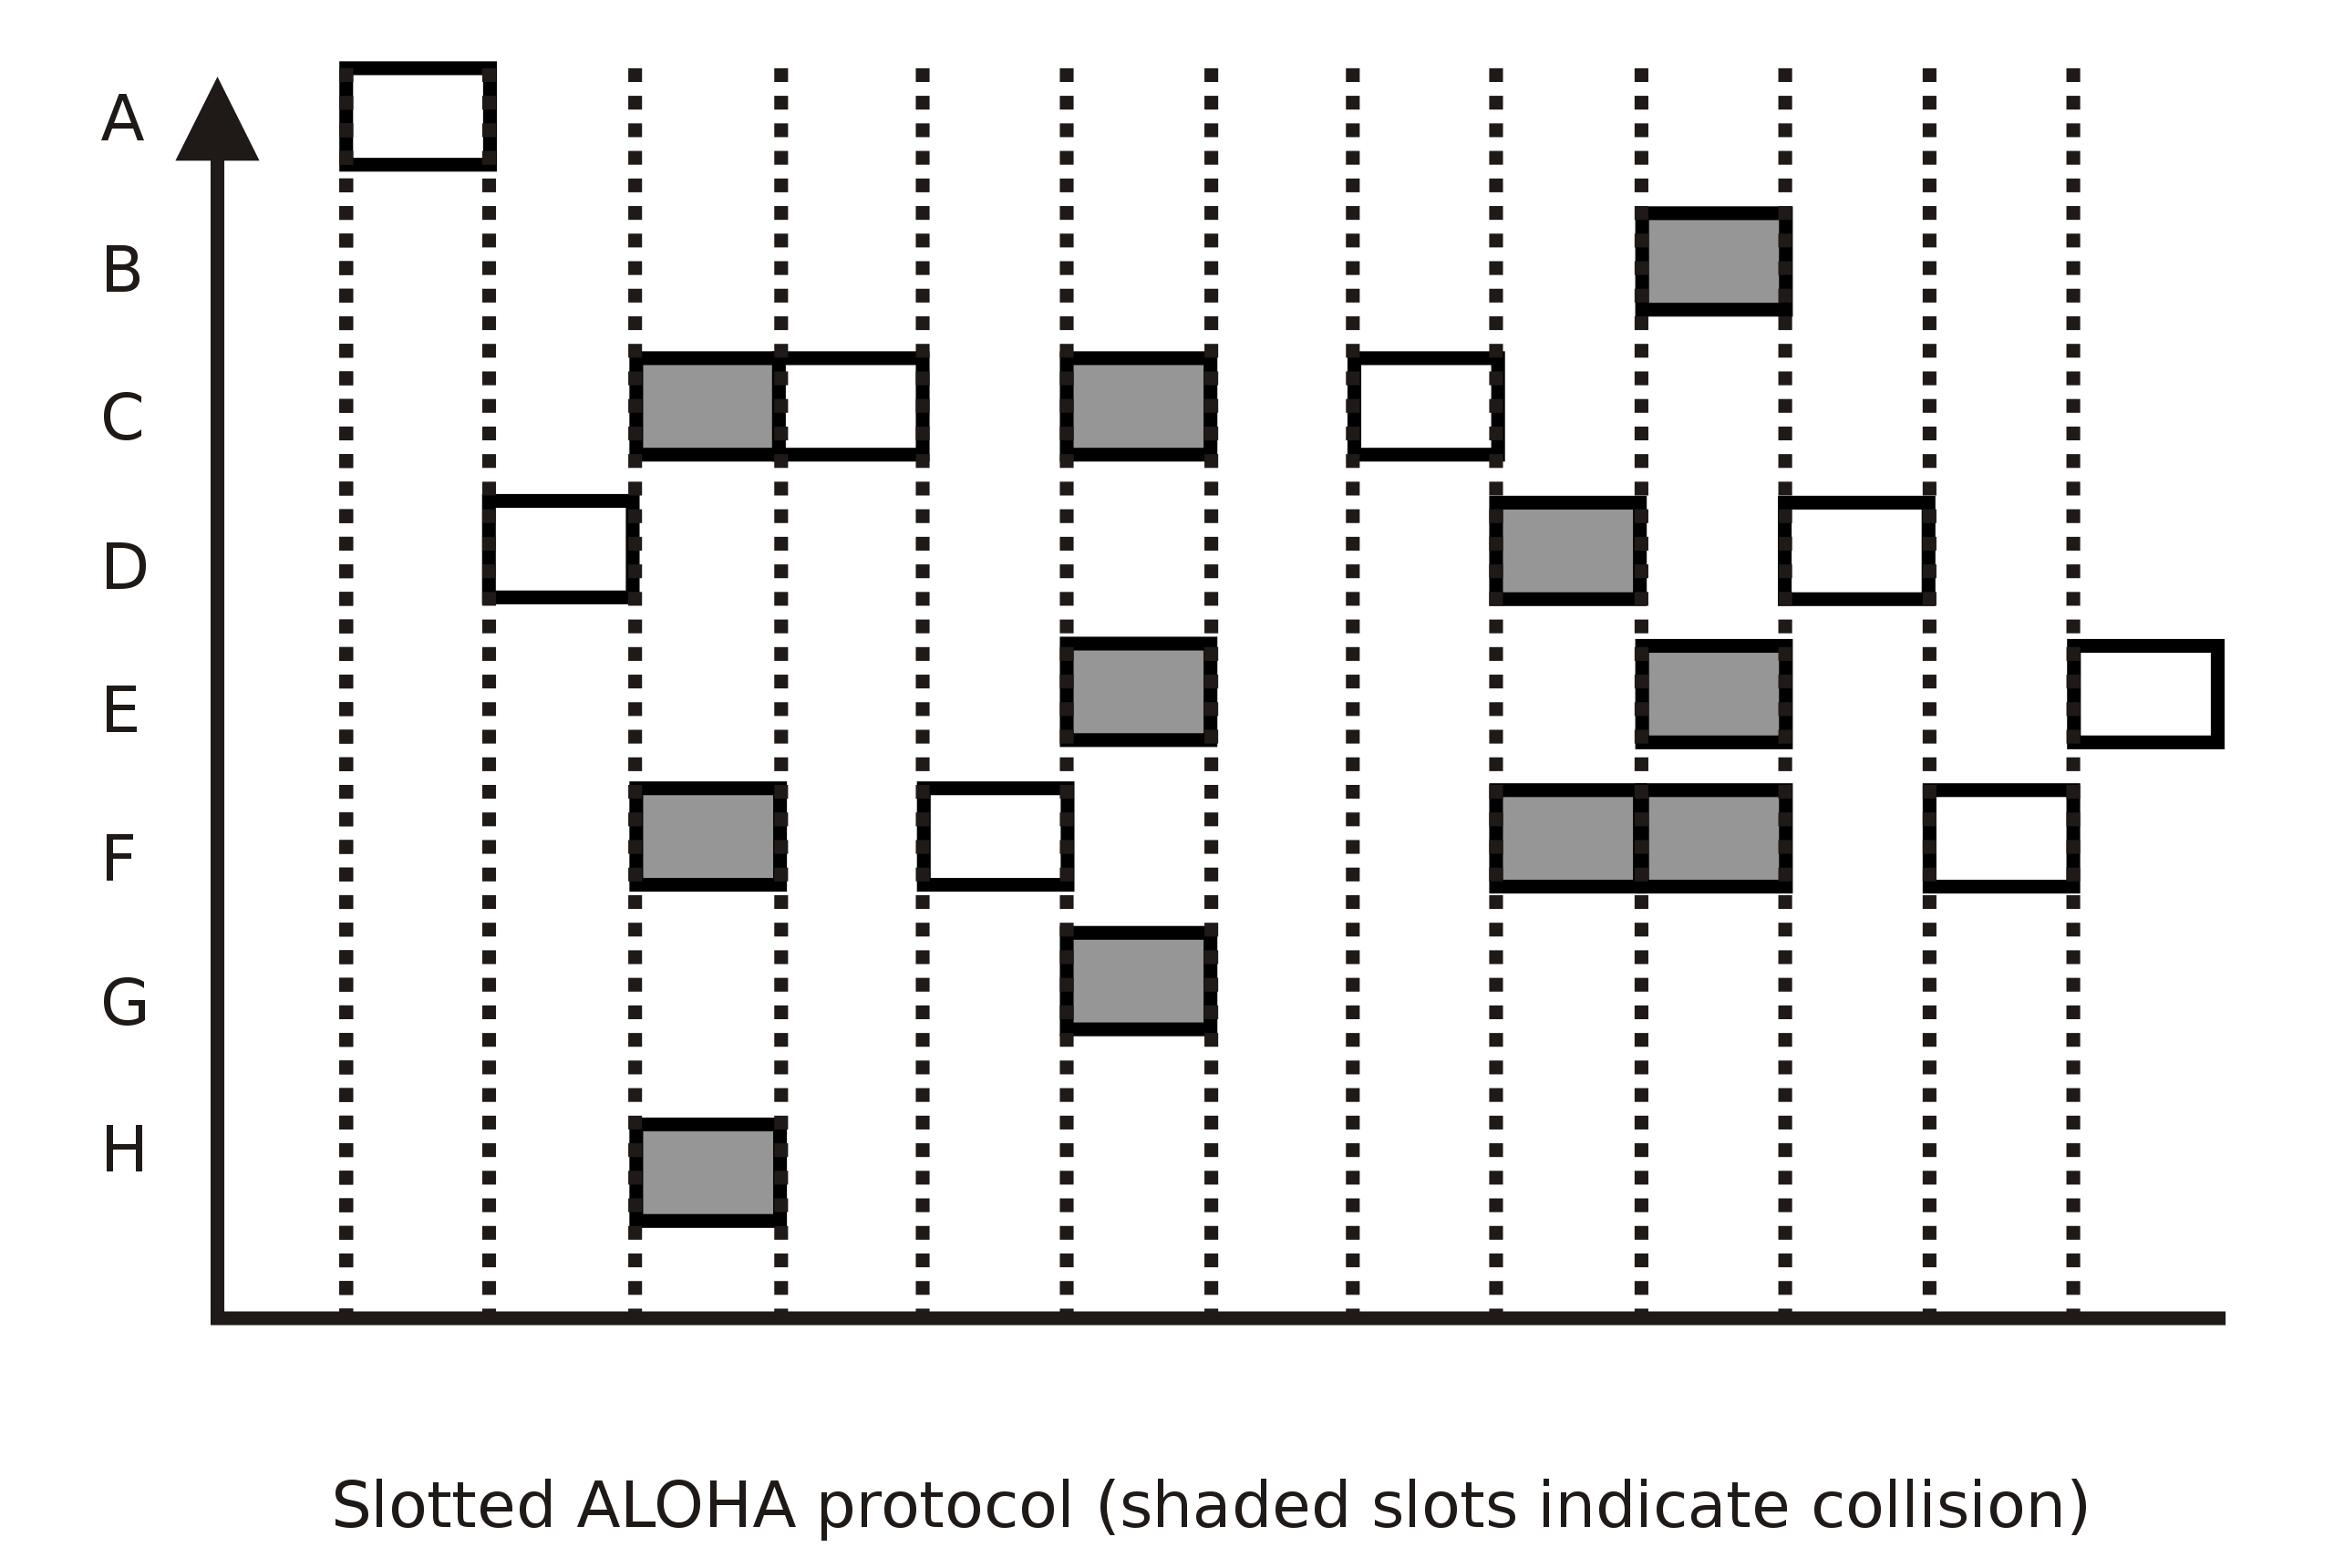
\includegraphics[width=0.6\textwidth]{assets/chap_4/slotted_aloha.png}
\end{figure}
\medskip

\begin{itemize}
    \item \textbf{Nguyên lý hoạt động:} thời gian được chia thành các khe (slots) có độ dài cố định ngang với thời gian truyền một gói tin (packet). \begin{itemize}
        \item Các trạm chỉ được phép bắt đầu gửi tại thời điểm bắt đầu của một slot.
        \item[$\Rightarrow$] Yêu cầu phải đồng bộ hóa thời gian chung (common time-base for synchronization).
    \end{itemize}
    \item \textbf{Ưu điểm (so với pure ALOHA):} collision chi xảy ra hoàn toàn (complete collision - trùng khít cả slot) chứ không bị chồng lên một phần $\rightarrow$ giảm xác suất lỗi; thông lượng (throughput) được cải thiện.
    \item \textbf{Nhược điểm:} chưa đảm bảo được fairness; delay tăng do phải chờ đến đầu slot tiếp theo thì mới được gửi.
\end{itemize}
\medskip

\noindent
$\Rightarrow$ Được dùng trong GSM network (Global System for Mobile Communications - mạng di động thế hệ đầu tiên).
\medskip

\subsubsection{Performance of ALOHA}

\begin{figure}[h]
    \centering
    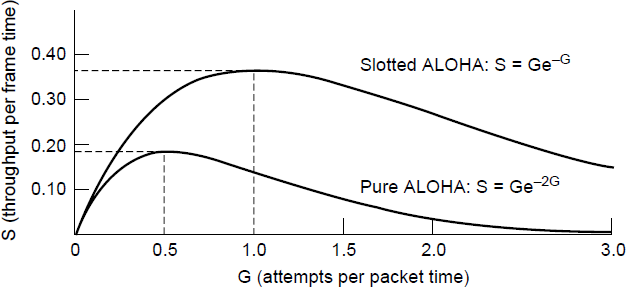
\includegraphics[width=0.8\textwidth]{assets/chap_4/performance_aloha.png}
\end{figure}
\medskip

\noindent
Để đánh giá hiệu suất của ALOHA, người ta sử dụng 2 thông số chính:

\begin{itemize}
    \item $S$ (throughput) $\rightarrow$ lượng dữ liệu truyền được thành công trên đơn vị thời gian.
    \item $G$ (load) $\rightarrow$ tổng lượng dữ liệu mà các trạm cố gắng gửi gói tin (bao gồm cả các gói tin bị collision) trên đơn vị thời gian.
\end{itemize}
\medskip

\noindent
\textbf{Pure ALOHA:} $\rightarrow$ protocol có hiệu suất thấp nhất.

\begin{itemize}
    \item \textbf{Công thức:} $S = G \cdot e^{-2G}$.
    \item \textbf{Hiệu suất tối đa:} đạt chỉ $\approx$18.4\% ($1/(2e)$) dung lượng kênh truyền (channel's capacity) $\Rightarrow$ đạt được khi $G = 0.5$ (nghĩa là trung bình cứ 2 khoảng thời gian truyền thì có 1 gói tin được gửi thành công).
    \item[$\Rightarrow$] \textbf{Lý do:} vì các trạm gửi tự do bất cứ lúc nào $\rightarrow$ kể cả một cái collision nhỏ cũng làm hỏng gói tin.
\end{itemize}
\medskip

\noindent
\textbf{Slotted ALOHA:} $\rightarrow$ cải tiến hiệu suất bằng cách ép buộc các trạm chỉ gửi ở đầu mỗi slot (do phải sync thời gian).

\begin{itemize}
    \item \textbf{Công thức:} $S = G \cdot e^{-G}$.
    \item \textbf{Hiệu suất tối đa:} đạt chỉ $\approx$37\% ($1/e$) dung lượng kênh truyền $\Rightarrow$ đạt được khi $G = 1$ (nghĩa là trung bình cứ 1 khoảng thời gian truyền thì có 1 gói tin được gửi thành công).
    \item[$\Rightarrow$] Slotted ALOHA cho throughput cao gấp đôi so với pure ALOHA $\Rightarrow$ nó phải đánh đổi bằng delay cao $\rightarrow$ phải chờ đến đầu slot tiếp theo mới được gửi.
\end{itemize}
\medskip

\noindent
\underline{Self-note:} cái hiệu suất nó mang tính "trong tổng số G attempt gửi đi thì có bao nhiêu phần trăm là may mắn không bị collision".

$\rightarrow$ Dùng Poisson để tính xác suất lần thử thành công: $S = G \cdot P$ (vì mô hình này giả định số lượng trạm tham gia rất lớn).

\begin{itemize}
    \item[$\rightarrow$] Với pure ALOHA: xác suất để không có trạm nào gửi tin trong khoảng thời gian $2t$ (tương ứng $2G$) $\rightarrow$ $P = e^{-2G}$.
    \item[$\rightarrow$] Với slotted ALOHA: xác suất để không có trạm nào gửi tin trong khoảng thời gian $t$ (tương ứng $G$) $\rightarrow$ $P = e^{-G}$.
\end{itemize}
\medskip

\noindent
$\Rightarrow$ Từ đây có thể thấy được slotted ALOHA giảm phân nửa khoảng thời gian collision.
\medskip

\subsection{CSMA}

\subsubsection{CSMA}

\noindent
CSMA $\rightarrow$ \textbf{C}arrier \textbf{S}ense \textbf{M}ultiple \textbf{A}ccess $\rightarrow$ hooạt động dựa trên nguyên tắc "nghe trước khi nói" (listen before talk).
\medskip

\noindent
\textbf{Nguyên lý hoạt động:} trạm phát phải lắng nghe (sense) đường truyền.

\begin{itemize}
    \item Nếu đường truyền bận (busy) $\rightarrow$ trạm phải đợi.
    \item Nếu đường truyền rảnh (idle) $\rightarrow$ trạm mới xem xét gửi dữ liệu.
\end{itemize}
\medskip

\noindent
Có 2 phương pháp chính để thực hiện CSMA.
\medskip

\noindent
\textbf{p-persistent CSMA (kiên trì xác suất p):}

\begin{itemize}
    \item Khi đường truyền bận $\rightarrow$ trạm tiếp tục đợi cho đến khi rảnh.
    \item Khi đường truyền rảnh $\rightarrow$ trạm gửi gói tin với xác suất $p$, hoặc phải chờ đến slot tiếp theo với xác suất $1-p$.
\end{itemize}
\medskip

\noindent
\underline{Self-note:} gửi $p$ xác suất ở đây như trò tung đồng xu $\rightarrow$ thấy đường dây rảnh thì bắt đầu random $\Rightarrow$ nếu rơi vào mặt ngửa ($p$) thì gửi, còn rơi vào mặt sấp ($1-p$) thì đợi đến slot tiếp theo rồi random lại $\rightarrow$ nếu đang tung mà thấy đường dây có đứa khác gửi thì chờ đến slot tiếp theo rồi random tiếp.
\medskip

$\Rightarrow$ Sẽ có lúc bị collision do dính xác suất cả 2 cùng chọn gửi trong cùng 1 slot, hoặc có thể bị delay do cả 2 đứa đều chờ mà nguyên đường dây không đứa nào gửi.
\medskip

\noindent
\textbf{Non-persistent CSMA (không kiên trì):}

\begin{itemize}
    \item Khi đường truyền bận $\rightarrow$ trạm không ngồi nghe liên tục mà sẽ đợi một khoảng thời gian ngẫu nghiên $\rightarrow$ sau đó quay lại nghe tiếp.
    \item Khi đường truyền rảnh $\rightarrow$ gửi gói tin ngay lập tức.
\end{itemize}
\medskip

\subsubsection{Performance of CSMA}

\begin{figure}[h]
    \centering
    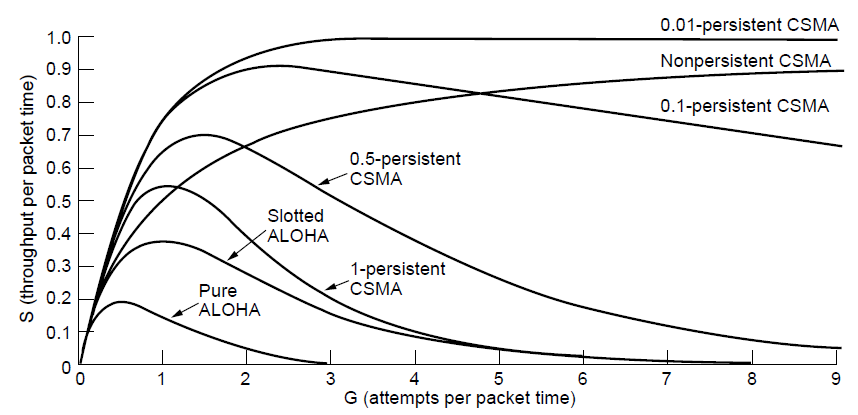
\includegraphics[width=0.8\textwidth]{assets/chap_4/performance_csma.png}
\end{figure}
\medskip

\noindent
Theo đồ thị biểu diễn hiệu suất của các phương pháp $\rightarrow$ cơ chế carrier sense giúp giảm xung đột đáng kể $\Rightarrow$ tăng dữ liệu truyền thành công cao hơn so với việc giử tự do như ALOHA.
\medskip

\noindent
\textbf{Với CSMA:}

\begin{itemize}
    \item \textbf{Hiệu suất cao} $\rightarrow$ $p$ càng nhỏ càng giúp tránh collision tốt hơn vì các trạm nhường nhau.
    \item \textbf{Delay cao} $\rightarrow$ do $p$ nhỏ $\rightarrow$ xác suất gửi đi thấp $\Rightarrow$ gói tin phải chờ rất lâu mới được gửi đi dù đường truyền trống.
\end{itemize}
\medskip

\pagebreak

\noindent
\underline{Self-note:} non-persistent khác với 1-persistent:

\begin{itemize}
    \item \textbf{Non-persistent:} đường truyền đợi một khoảng thời gian random rồi mới nghe lại $\rightarrow$ nếu đường truyền rảnh thì gửi ngay.
    \item \textbf{1-persistent:} đường truyền cứ nghe liên tục đến khi rảnh thì gửi ngay.
\end{itemize}
\medskip

\subsection{CSMA/CA and MACA}

\subsubsection{CSMA/CA}

\noindent
$\rightarrow$ Tránh xung đột (collision avoidance) thay vì phát hiện xung đột (collision detection).
\medskip

\vspace{0.3cm}

\noindent
\textbf{Tại sao không dùng CSMA/CD (collision detection)?}

\begin{itemize}
    \item Trong mạng không dây $\rightarrow$ việc vừa gửi vừa nghe để bắt xung đột là rất khó $\Rightarrow$ vì trạm phát ra một tín hiệu rất mạnh $\rightarrow$ át hoàn toàn các tín hiệu yếu hơn từ xa tới $\rightarrow$ máy không thể biết gói tin có bị collision không.
    \item Có vấn đề trạm ẩn (hidden terminal) $\rightarrow$ các trạm không nghe thấy nhau dẫn đến việc gửi cùng lúc với nhau $\rightarrow$ gây ra xung đột.
\end{itemize}
\medskip

\noindent
$\Rightarrow$ Chính vì không thể phát hiện xung đột $\rightarrow$ chọn cách tránh xung đột ngay từ đầu là hợp lý nhất.
\medskip

\noindent
\textbf{Ở sender:}

\begin{itemize}
    \item Nếu thấy đường truyền rảnh $\rightarrow$ nó không gửi ngay mà chờ thêm một khoảng thời gian (time slots/DIFS - Distributed Interframe Space) để chắc chắn rồi mới gửi.
    \item Dựa vào ACK (acknowledgment) để biết $\rightarrow$ do sender không tự biết có lỗi hay không $\rightarrow$ phụ thuộc hoàn toàn vào response của receiver. \begin{itemize}
        \item[$\Rightarrow$] Nếu gửi xong mà không nhận được ACK $\rightarrow$ sender tự hiểu là bị mất hoặc collision $\rightarrow$ nó sẽ gửi lại (retransmit).
    \end{itemize}
\end{itemize}
\medskip

\noindent
\textbf{Ở receiver:}

\begin{itemize}
    \item Khi nhận được gói tin $\rightarrow$ kiểm tra xem có lỗi không (dùng checksum/CRC).
    \item Nếu gói tin error-free $\rightarrow$ receiver sẽ đợi một khoảng thời gian ngắn (short time delay/SIFS - Short Interframe Space) $\rightarrow$ gửi ACK trở lại cho sender.
\end{itemize}
\medskip

\noindent
$\Rightarrow$ Mạng không dây không thấy được trạm ẩn khi phát sóng, và không thấy được collision $\rightarrow$ nó không thể tự bắt lỗi được $\rightarrow$ phải dựa vào ACK từ receiver để biết có lỗi hay không.
\medskip

\pagebreak

\subsubsection{Functioning of CSMA/CA}

\begin{figure}[h]
    \centering
    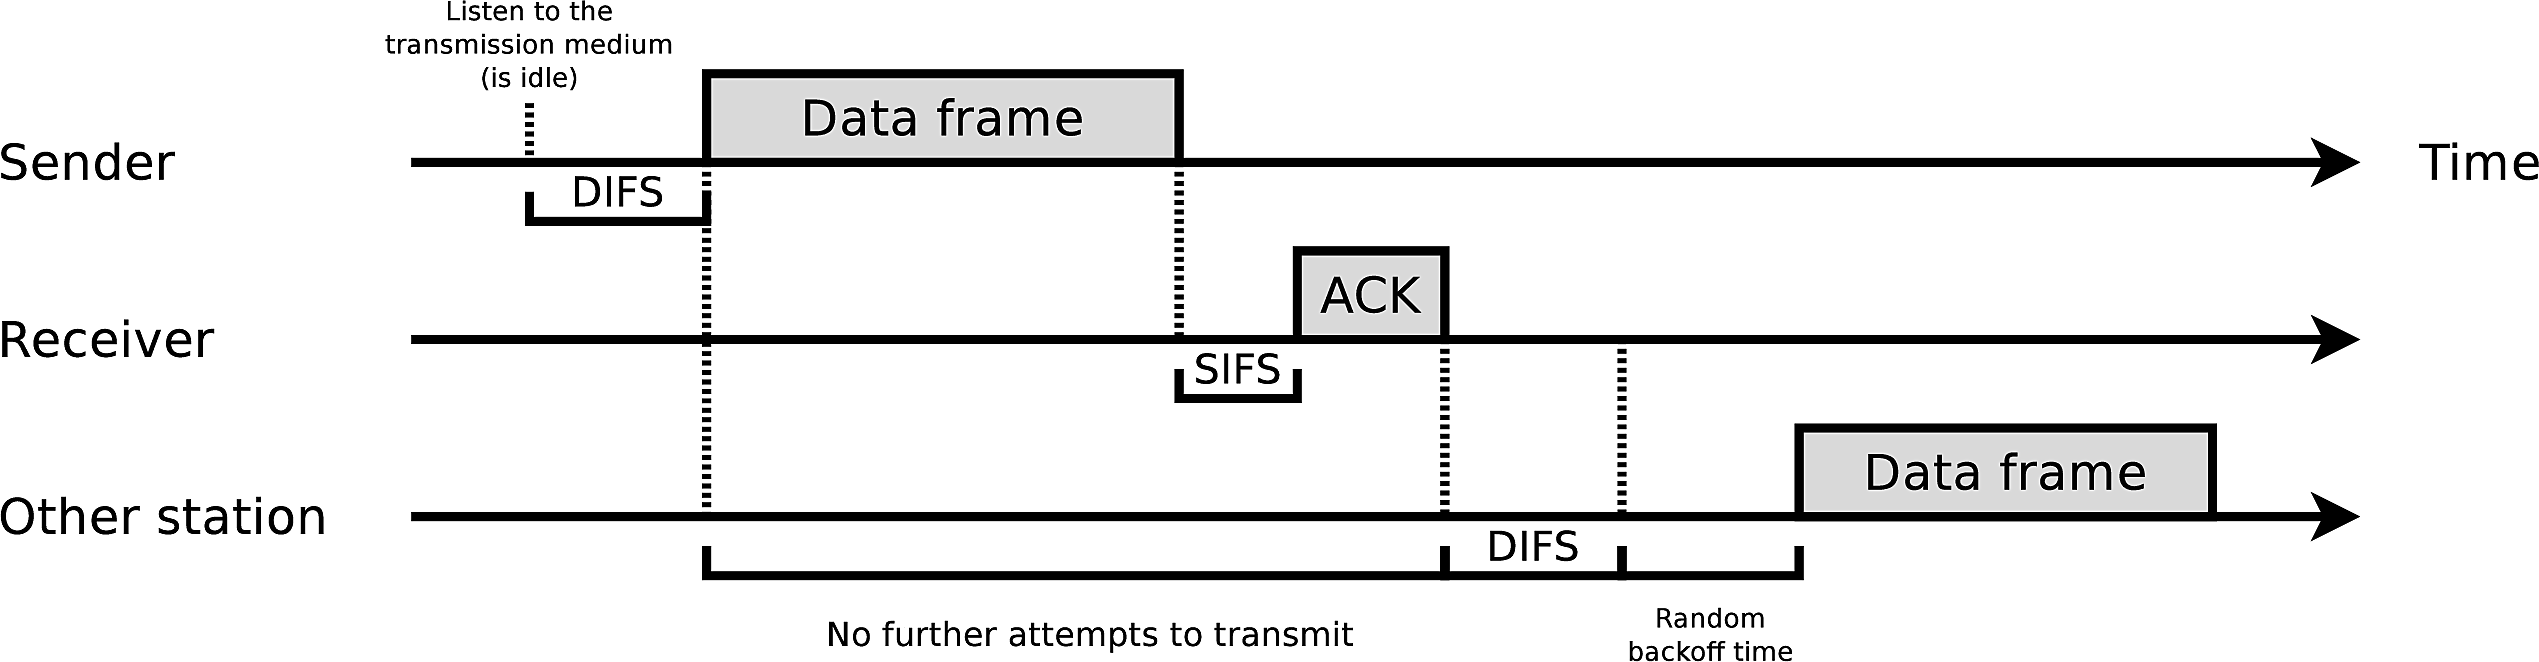
\includegraphics[width=0.9\textwidth]{assets/chap_4/csma_functioning.png}
\end{figure}
\medskip

\noindent
\textbf{Ở sender:}
\medskip

\noindent
Đầu tiên, sender lắng nghe kênh truyền ($\rightarrow$ carrier sense) $\rightarrow$ kênh truyền cẩn phải không có tín hiệu trong một khoảng thời gian ngắn.

$\Rightarrow$ Khoảng thời gian này được gọi là DIFS (Distributed Interframe Space) $\approx$50$\mu$s.
\medskip

\noindent
$\rightarrow$ Nếu kênh truyền không có tín hiệu trong suốt 1 DIFS $\rightarrow$ trạm có thể bắt đầu gửi frame.
\medskip

\vspace{0.3cm}

\noindent
\textbf{Ở receiver:}
\medskip

\noindent
Nếu trạm nhận được success frame (đã pass CRC check) $\rightarrow$ nó sẽ đợi một khoảng thời gian ngắn.

$\Rightarrow$ Khoảng thời gian này được gọi là SIFS (Short Interframe Space) $\approx$10$\mu$s.
\medskip

\noindent
Sau đó, receiver gửi một acknowledgment frame (ACK).
\medskip

\noindent
$\Rightarrow$ DIFS và SIFS đảm bảo được khoảng cách tối thiểu cho CSMA/CA khi một chuỗi frame sẽ được gửi.
\medskip

\vspace{0.3cm}

\noindent
\textbf{Random backoff (tranh chấp ngẫu nhiên):}
\medskip

\noindent
$\rightarrow$ Nếu sau khi chờ DIFS mà có nhiều trạm cùng muốn gửi, hoặc đường truyền đang bận $\rightarrow$ cơ chế random backoff sẽ được kích hoạt để tránh va chạm.
\medskip

\noindent
Backoff calculation $\rightarrow$ sender sẽ chọn một giá trị ngẫu nhiên (nằm trong khoảng min và max của contention window - CW) $\rightarrow$ đem nhân với thời gian của một slot $\Rightarrow$ sender bắt đầu đếm ngược thời gian này.

$\Rightarrow$ Nếu backoff time kết thúc $\rightarrow$ sender được phép gửi frame.
\medskip

\noindent
Nếu trong thời gian backoff mà có một trạm khác nhảy vào chiếm đường truyền $\rightarrow$ sender sẽ dừng đếm (the counter variable is stopped).

$\rightarrow$ Đợi cho đến khi đường truyền rảnh trở lại trong ít nhất 1 DIFS $\rightarrow$ tiếp tục đếm ngược giá trị backoff còn lại.
\medskip

\pagebreak

\noindent
\underline{Self-note:} \textit{(Tóm tắt)}

\begin{itemize}
    \item Muốn gửi data $\rightarrow$ phải chờ DIFS $\Rightarrow$ tốn thời gian hơn.
    \item Muốn gửi ACK $\rightarrow$ chỉ cần chờ SIFS $\Rightarrow$ nhanh hơn vì ACK được ưu tiên chạy trước.
    \item Nếu đường bận $\rightarrow$ chọn random backoff time để xếp hàng chờ gửi $\Rightarrow$ nếu có đứa nào chen vào thì dừng đếm, chờ DIFS, rồi đếm tiếp.
\end{itemize}
\medskip

\subsubsection{MACA (Multiple Access with Collision Avoidance)}

\noindent
CSMA/CA giảm thiểu collision $\rightarrow$ nhưng không thể loại bỏ hoàn toàn.

$\Rightarrow$ MACA/MACAW là phiên bản nâng cấp của CSMA/CA $\rightarrow$ được thiết kế đặc biệt để giải quyết bài toán trạm ẩn (hidden terminal problem) mà CSMA/CA không xử lý triệt để được.
\medskip

\noindent
MACAW $\rightarrow$ \textbf{M}ultiple \textbf{A}ccess with \textbf{C}ollision \textbf{A}voidance for \textbf{W}ireless $\Rightarrow$ là phiên bản mở rộng của MACA $\rightarrow$ bổ sung thêm một số tính năng để cải thiện hiệu suất và độ tin cậy.
\medskip

\vspace{0.3cm}

\noindent
\textbf{Nguyên lý hoạt động:}
\medskip

\noindent
Thay vì chỉ nghe và gửi như CSMA/CA $\rightarrow$ MACA yêu cầu sender và receiver phải trao các frame điều khiển (control frames) trước khi gửi dữ liệu.

$\Rightarrow$ Nhờ cách này mà tất cả các trạm trong mạng đều biết rằng sắp có một phiên truyền (transmission) bắt đầu $\rightarrow$ tránh được việc truy cập đồng thời.
\medskip

\noindent
Các frame điểu khiển bao gồm \textbf{RTS} (Request to Send - yêu cầu gửi) và \textbf{CTS} (Clear to Send - cho phép gửi).

$\Rightarrow$ Những khung này chứa thông tin về khoảng thời gian kênh truyền sẽ bị sử dụng (occupation time of the channel).
\medskip

\begin{figure}[h]
    \centering
    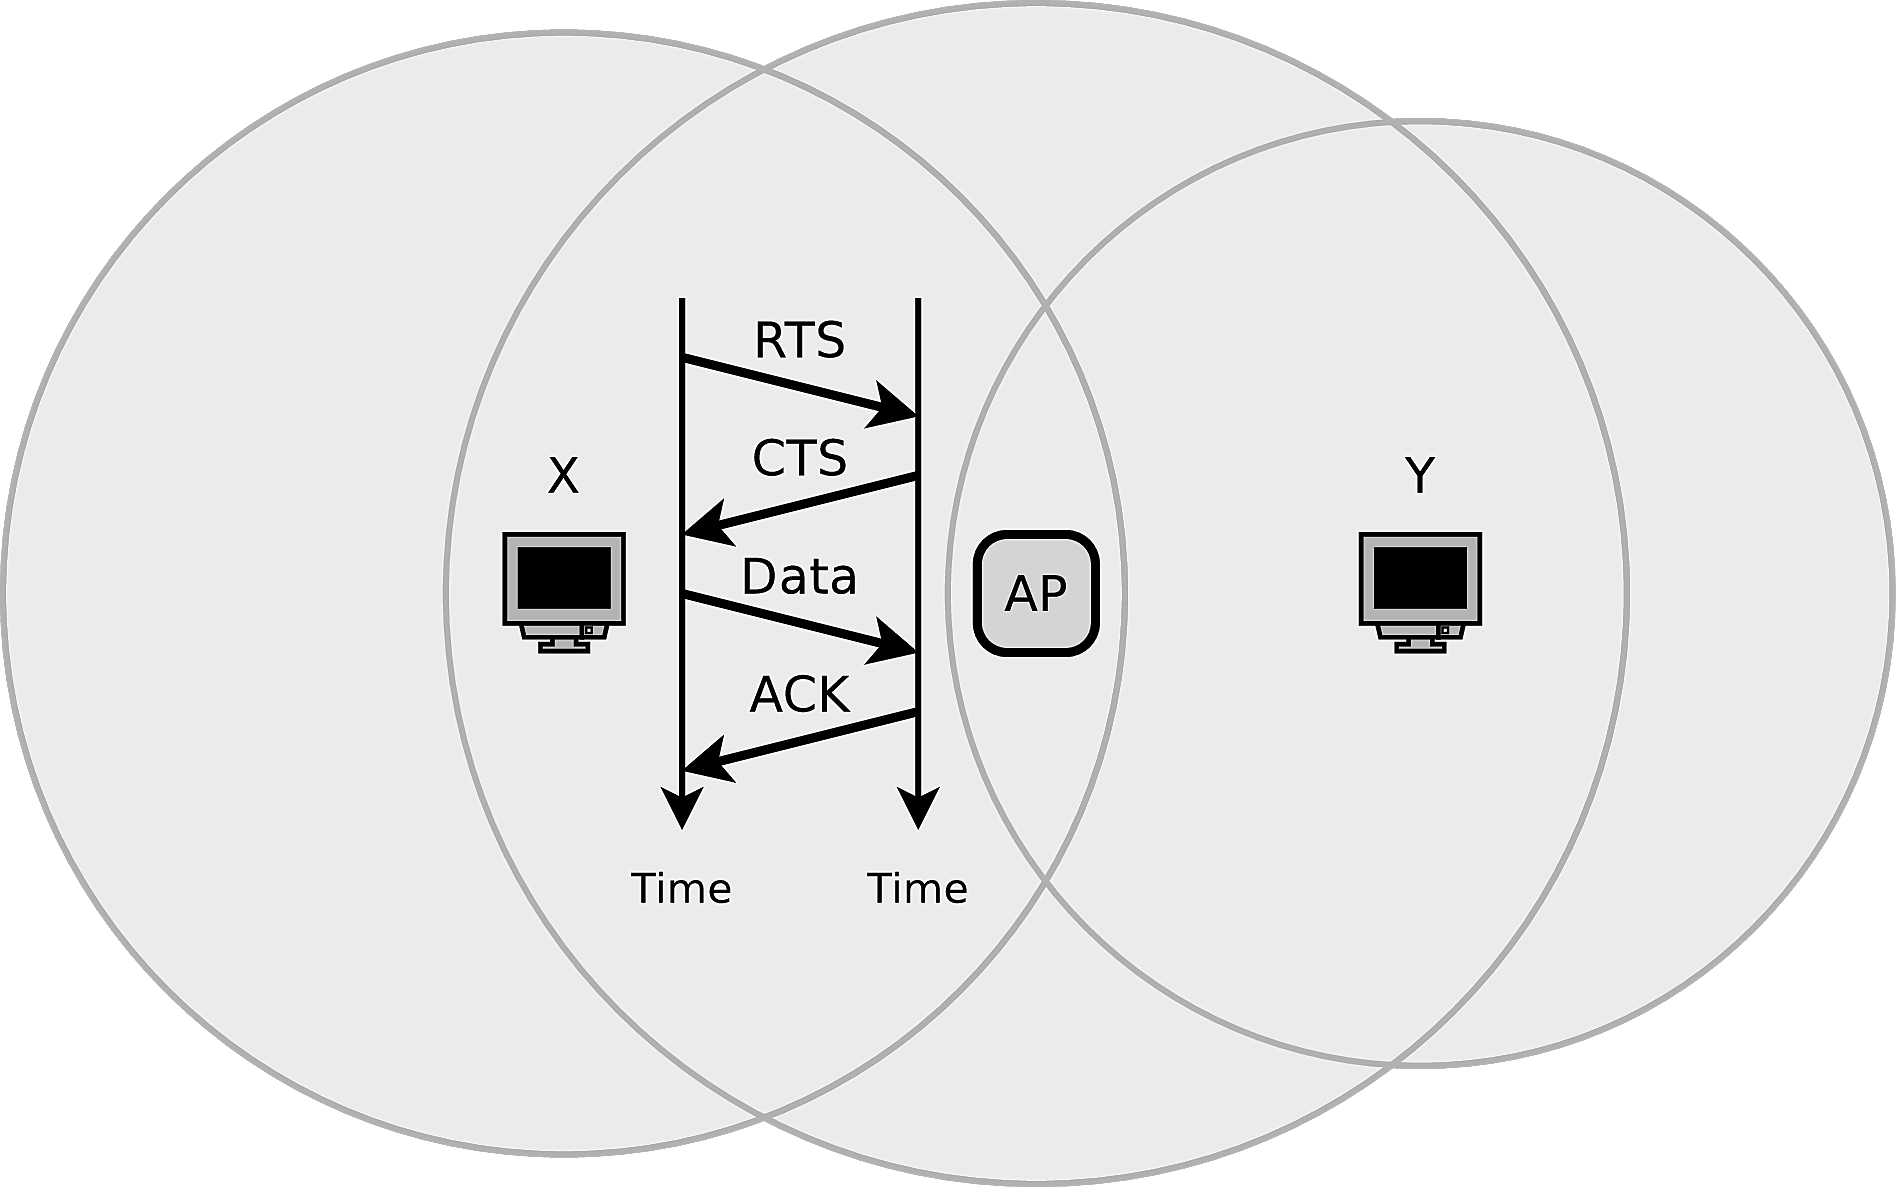
\includegraphics[width=0.5\textwidth]{assets/chap_4/maca_dia.png}
\end{figure}
\medskip

$\Rightarrow$ Theo hình trên: trạm Y không nhận được RTS frame do trạm X gửi $\rightarrow$ nhưng vẫn nhận được tín hiệu cho phép gửi (CTS) phát ra từ access point (AP).
\medskip

\noindent
$\rightarrow$ Collision chỉ có thể xảy ra trong quá trình truyền các frame RTS và CTS $\rightarrow$ do ảnh hưởng của hidden terminal.
\medskip

\subsubsection{Functioning of MACA}

\begin{figure}[h]
    \centering
    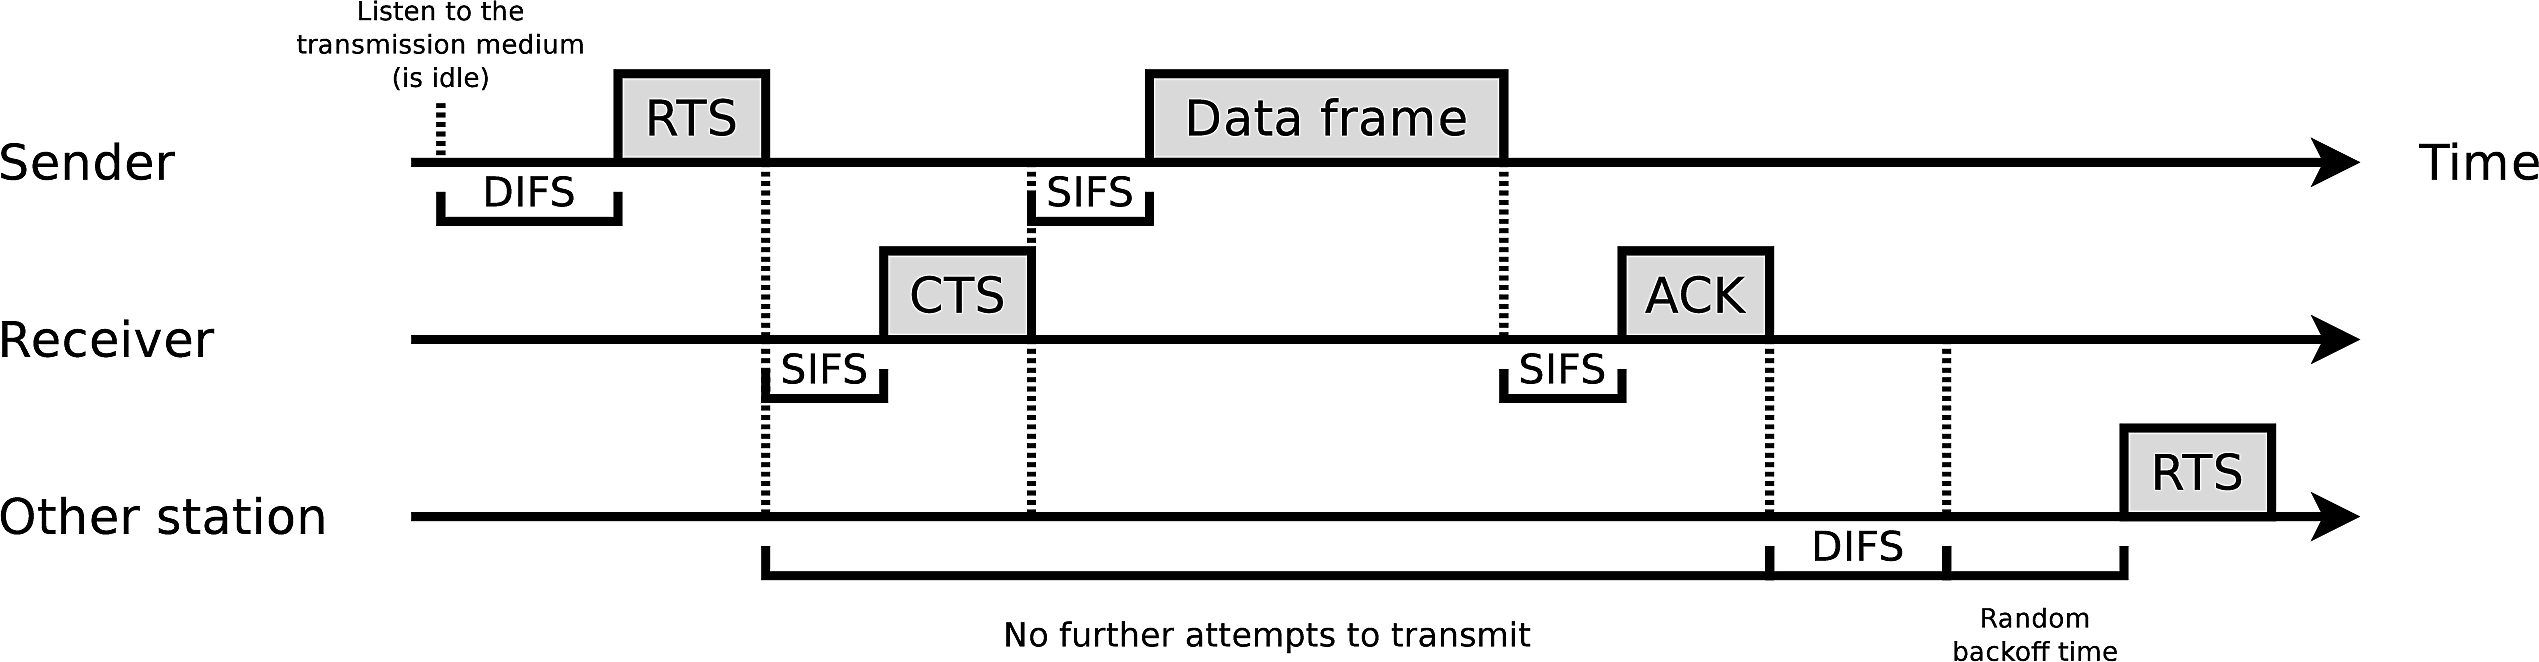
\includegraphics[width=0.9\textwidth]{assets/chap_4/maca_functioning.png}
\end{figure}
\medskip

\noindent
\textbf{Ở sender:}
\medskip

\noindent
Đầu tiên, sender lắng nghe kênh truyền $\rightarrow$ sau khoảng thời gian DIFS, sender gửi một RTS frame đến receiver.
\medskip

\vspace{0.3cm}

\noindent
\textbf{Ở receiver:}
\medskip

\noindent
$\rightarrow$ Xác nhận yêu cầu sử dụng kênh (reservation request) $\rightarrow$ chờ một khoảng thời gian SIFS $\rightarrow$ gửi lại (transmit) một CTS frame chứa khoảng thời gian mà sender muốn dành riêng để sử dụng transmission medium.
\medskip

\vspace{0.3cm}

\noindent
$\Rightarrow$ Sau khi receiver nhận thành công dữ data frame $\rightarrow$ nó sẽ chờ một khoảng thời gian SIFS $\rightarrow$ gửi ACK trở lại cho sender.
\medskip

\vspace{0.3cm}

\noindent
Khi transmission medium bận (occupied) $\rightarrow$ các trạm khác sẽ không cố để truyền data frame mới cho đến khi NAV (Network Allocation Vector - bộ đếm thời gian dành riêng cho kênh) kết thúc.
\medskip

\vspace{0.3cm}

\noindent
\textbf{Cơ chế NAV:}

\begin{itemize}
    \item NAV $\rightarrow$ là một biến đếm mà mỗi trạm tự quản lý.
    \item \textbf{Chức năng:} chứa thông tin về thời gian dự kiến mà đường truyền sẽ bị sử dụng.
    \item \textbf{Nguyên lý hoạt động:} \begin{itemize}
        \item Khi các trạm khác nghe thấy RTS hoặc CTS (có chứa thông tin thời gian) $\rightarrow$ chúng sẽ cập nhật vào NAV của chính mình.
        \item Biến NAV sẽ tự động giảm dần cho đến khi về 0.
        \item Trong khoảng thời gian NAV chưa về 0 $\rightarrow$ các trạm sẽ không tiếp tục gửi bất cứ thứ gì (no further attempts to transmit).
    \end{itemize}
    \item[$\Rightarrow$] Giảm thiểu được số lượng xung đột.
\end{itemize}
\medskip

\noindent
\begin{itemize}
    \item \textbf{Pros:} \begin{itemize}
        \item Ít bị xung đột hơn $\rightarrow$ giải quyết triệt để vấn đề trạm ẩn ($\rightarrow$ xung đột chỉ có thể xảy ra ở bước RTS/CTS rất ngắn).
        \item Tiết kiệm năng lượng hơn $\rightarrow$ các trạm khác không cần tốn năng lượng để gửi tin trong thời gian NAV.
    \end{itemize}
    \item \textbf{Cons:} \begin{itemize}
        \item Gây delay cao $\rightarrow$ việc phải xin phép RTS/CTS gây tốn thời gian.
        \item Tốn băng thông (overhead) $\rightarrow$ các gói tin RTS và CTS tuy nhỏ nhưng vẫn sử dụng đường truyền đáng kể.
    \end{itemize}
\end{itemize}
\medskip

\noindent
\underline{Self-note:} \textit{(Tóm gọn MACA functioning)}
\medskip

\noindent
Xin (RTS) $\rightarrow$ cho phép (CTS) $\rightarrow$ các bên khác im lặng (chờ NAV) $\rightarrow$ gửi data $\rightarrow$ gửi ACK.
\medskip

\section{Contention-free}

\subsection{Token Passing}

\begin{center}
\begin{minipage}[c]{0.6\textwidth}
    \textbf{Nguyên lý hoạt động:}
    \begin{itemize}
        \item Token frame $\rightarrow$ có một gói tin đặc biệt gọi là token $\rightarrow$ được truyền đi vòng quanh mạng (thường là cấu trúc dạng vòng - ring).
        \item[$\rightarrow$] Token này có tác dụng xác định thứ tự ai được phép gửi data (defining the sending order).
        \item \textbf{Quy luật:} chỉ có trạm nào đang giữ token thì mới có quyền gửi data ($\rightarrow$ eliminates collisions). \begin{itemize}
            \item Nếu trạm đó có dữ liệu cần gửi $\rightarrow$ nó giữ token, gửi data, rồi mới chuyển token cho trạm kế tiếp.
            \item Nếu trạm đó không có dữ liệu cần gửi $\rightarrow$ nó chuyển token ngay cho trạm kế tiếp.
        \end{itemize}
    \end{itemize}
\end{minipage}
\hfill
\begin{minipage}[c]{0.35\textwidth}
    \centering
    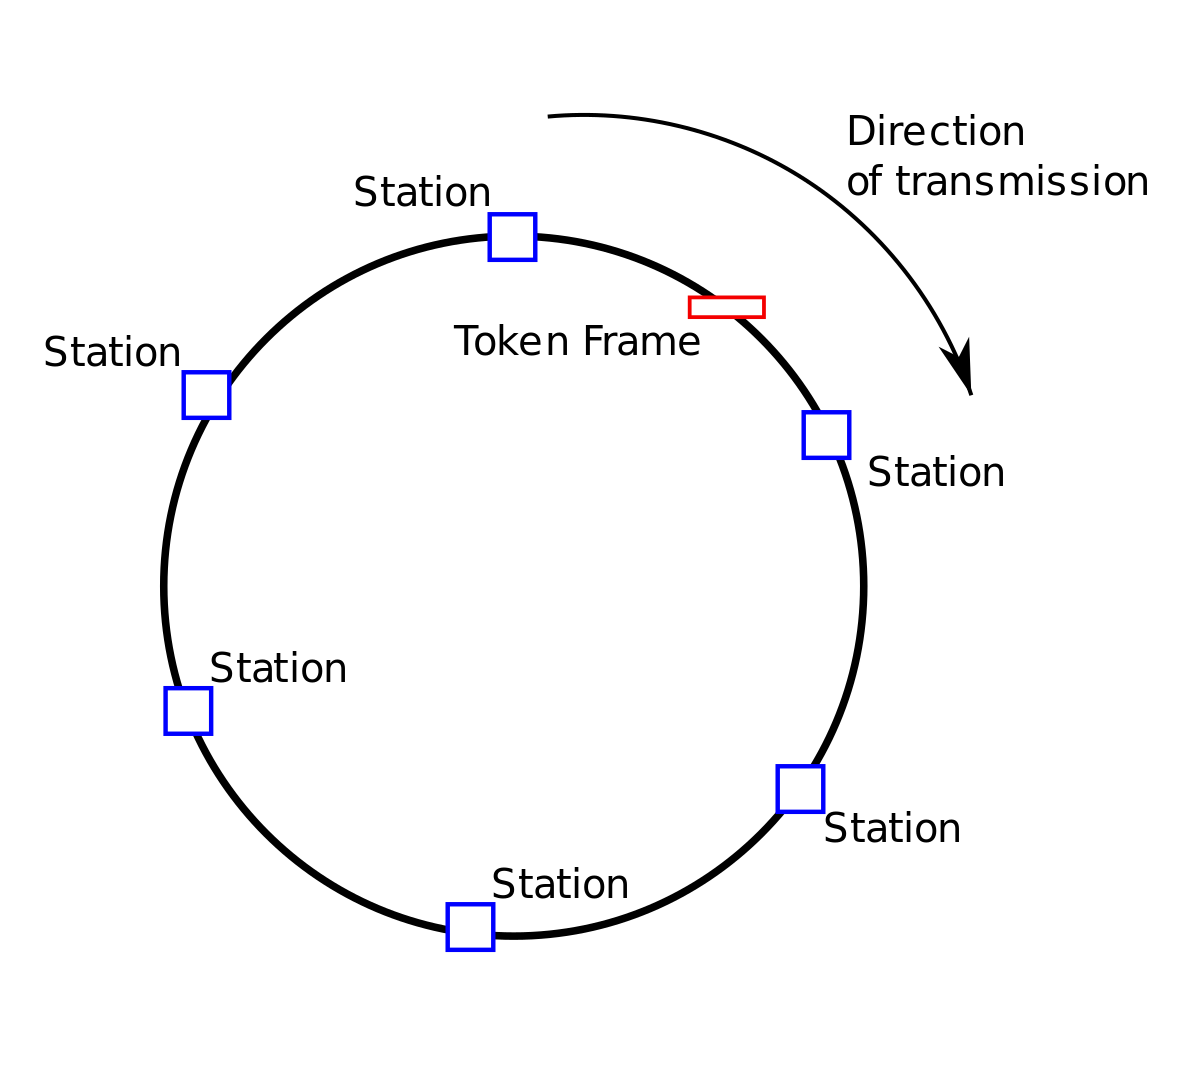
\includegraphics[width=1\textwidth]{assets/chap_4/token.png}
\end{minipage}
\end{center}
\medskip

\noindent
\textbf{Cấu trúc mạng (topology):} thường được hình dung trong cấu trúc mạng dạng vòng (ring) $\rightarrow$ nơi token đi từ trạm này sang trạm liền kề theo một chiều cố định.

$\Rightarrow$ Tuy nhiên, ý tưởng này cũng có thể áp dụng cho các cấu trúc khác; chẳng hạn như token bus.
\medskip

\subsection{TDMA}

\noindent
TDMA $\rightarrow$ \textbf{T}ime \textbf{D}ivision \textbf{M}ultiple \textbf{A}ccess $\rightarrow$ phân chia theo thời gian.
\medskip

\begin{figure}[h]
    \centering
    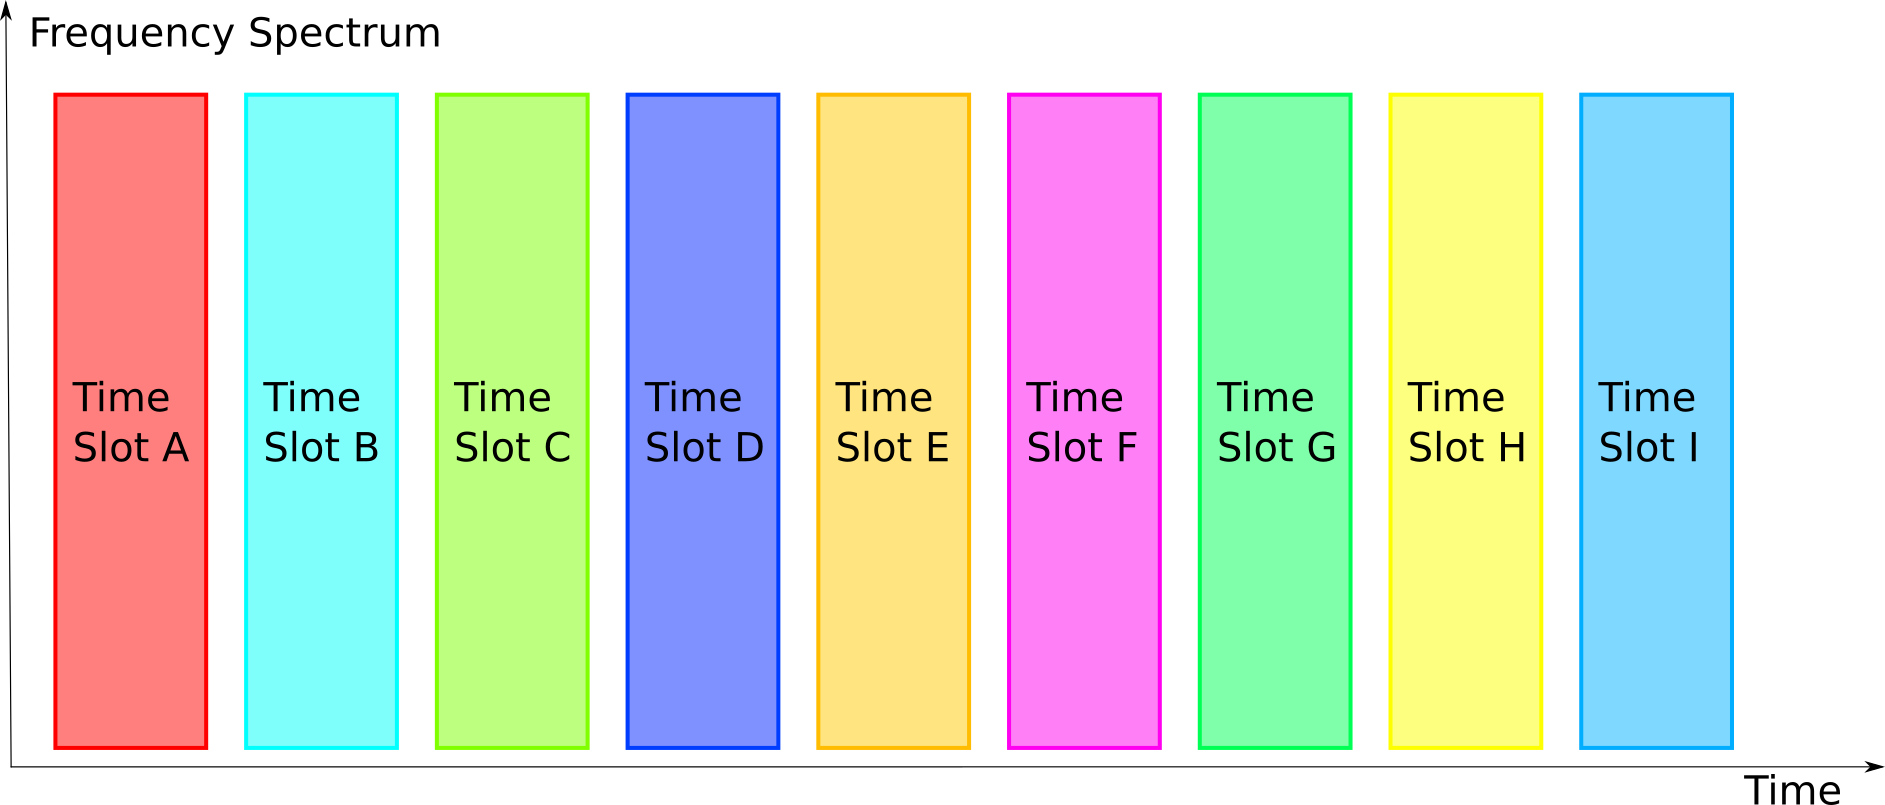
\includegraphics[width=0.6\textwidth]{assets/chap_4/tdma.png}
\end{figure}
\medskip

\noindent
$\rightarrow$ Tại một thời điểm, chỉ có 1 người dùng toàn bộ tần số $\rightarrow$ nhưng họ thay phiên nhau theo thời gian \textit{(hình minh họa trên)}.
\medskip

\vspace{0.3cm}

\noindent
\textbf{Nguyên lý hoạt động:}

\begin{itemize}
    \item Chia slot thời gian (time slots) $\rightarrow$ thời gian được chia nhỏ thành các slots.
    \item Phân quyền $\rightarrow$ mỗi time slot được gán cố định cho một máy chủ (host) cụ thể.
    \item[$\rightarrow$] Trong suốt thời gian của slot đó $\rightarrow$ máy chủ được quyền sử dụng toàn bộ dung lượng đường truyền (full channel capacity) $\Rightarrow$ không một máy nào được cắt ngang.
\end{itemize}
\medskip

\noindent
\textbf{Cách lên lịch (scheduling):} có thể thực hiện bằng 2 cách:

\begin{itemize}
    \item Static (tĩnh) $\rightarrow$ lịch cố định; ví dụ như A luôn gửi ở slot 1, B luôn gửi ở slot 2.
    \item Dynamic (động) $\rightarrow$ lịch thay đổi tùy theo nhu cầu thực tế.
\end{itemize}
\medskip

\noindent
$\Rightarrow$ \underline{Note:} một số time slot có thể được dành riêng cho broadcast traffic.
\medskip

\vspace{0.3cm}

\noindent
\underline{Self-note:} TDMA giống kiểu như chia nhau theo giờ, đến giờ của ai thì người đó dùng, dùng xong thì nhường cho người tiếp theo $\rightarrow$ tuy nhiên thì trong lúc dùng, mình được phép dùng hết công suất.
\medskip

\subsection{FDMA}

\subsubsection{Frequency Division Multiple Access (FDMA)}

\begin{figure}[h]
    \centering
    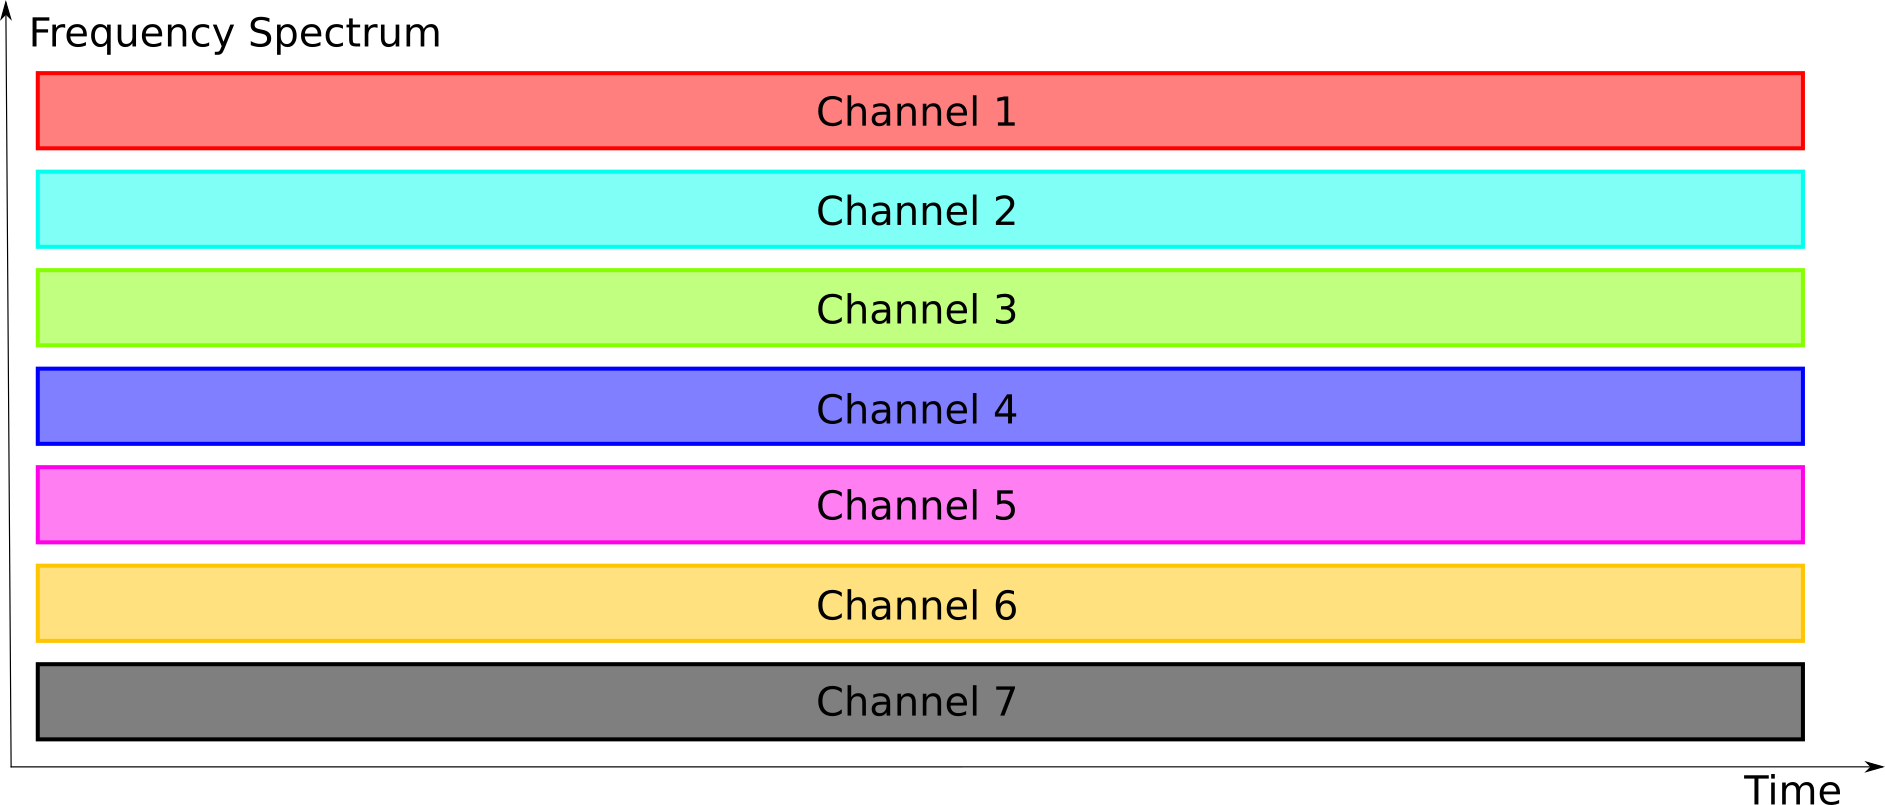
\includegraphics[width=0.6\textwidth]{assets/chap_4/fdma.png}
\end{figure}
\medskip

\noindent
$\rightarrow$ Chia thành các kênh con (sub-channels) riêng biệt $\rightarrow$ có thể hoạt động song song cùng một lúc với nhau \textit{(hình minh họa trên)}.
\medskip

\vspace{0.3cm}

\noindent
\textbf{Nguyên lý hoạt động:}

\begin{itemize}
    \item Chia nhỏ phổ tần (subdivide spectrum) $\rightarrow$ thay vì dùng toàn bộ băng thông $\rightarrow$ FDMA chia nhỏ dải tần số thành các kênh con (sub-channels) riêng biệt.
    \item Phân quyền $\rightarrow$ mỗi máy chủ (host) hoặc mỗi liên kết (link) được gán cho một kênh tần số riêng.
    \item[$\Rightarrow$] Mọi máy có thể truyền dữ liệu song song cùng một lúc (liên tục theo thời gian) $\rightarrow$ nhưng không lấn nhau do mỗi bên truyền ở mỗi tần số khác nhau.
\end{itemize}
\medskip

\noindent
\textbf{Quản lý kênh:}

\begin{itemize}
    \item Control traffic (kênh điều khiển) $\rightarrow$ thường được gửi trên các kênh cố định để đảm bảo kết nối.
    \item \textbf{Cách gán kênh:} \begin{itemize}
        \item Static (tĩnh) $\rightarrow$ gán kênh cố định; ví dụ như đài A luôn phát ở 100MHz, đài B luôn phát ở 105MHz.
        \item Dynamic (động) $\rightarrow$ kênh thay đổi theo nhu cầu sử dụng $\Rightarrow$ việc phân bổ này dẫn đến một vấn đề là "graph coloring problem" $\rightarrow$ làm sao để gán màu (tần số) cho các trạm cạnh nhau mà không bị trùng nhau.
    \end{itemize}
\end{itemize}
\medskip

\pagebreak

\noindent
\underline{Self-note:} \textit{(tổng kết lại)}
\medskip

\begin{itemize}
    \item TDMA $\rightarrow$ chia thời gian thành các time slots $\rightarrow$ mỗi time slot chỉ được 1 host sử dụng, và máy đó được dùng toàn bộ băng thông.
    \item FDMA $\rightarrow$ chia băng thông thành các sub-channels $\rightarrow$ tất cả các host đều hoạt động song song nhưng chỉ trong một dải băng tần nhất định, không lấn nhau.
\end{itemize}
\medskip

\subsubsection{Example: IEEE 802.15.4e}

\begin{figure}[h]
    \centering
    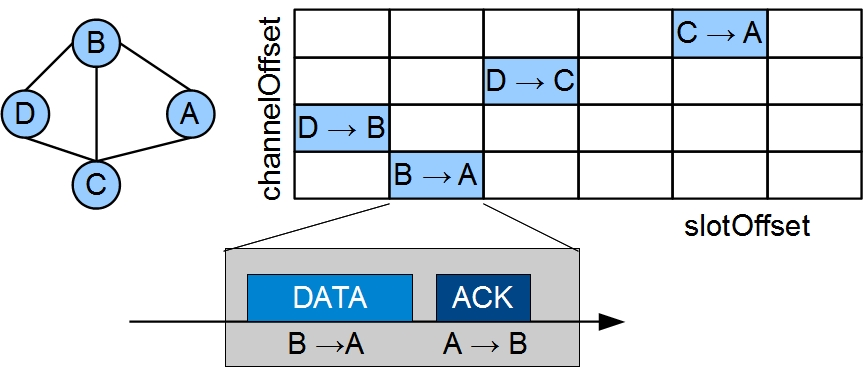
\includegraphics[width=0.6\textwidth]{assets/chap_4/ieee.jpg}
\end{figure}
\medskip

\noindent
$\rightarrow$ Là một tiêu chuẩn (specification) cho mạng cá nhân không dây (PAN); chẳng hạn như Zigbee.
\medskip

\vspace{0.3cm}

\noindent
Là một bản chỉnh sửa (amendment) của tầng MAC $\Rightarrow$ hỗ trợ cơ chế time-slotted channel hopping (TiSCH) dựa trên TDMA và FDMA \textit{(theo hình)}:

\begin{itemize}
    \item \textbf{Time-slotted (TDMA)} $\rightarrow$ trục hoành là thời gian \textit{(slotOffset)} $\rightarrow$ thời gian được chia thành các slot. \begin{itemize}
        \item[$\rightarrow$] Trong 1 slot, thiết bị sẽ làm trọn vẹn quy trình: gửi \texttt{DATA} $\rightarrow$ chờ $\rightarrow$ nhận \texttt{ACK}.
    \end{itemize}
    \item \textbf{Channel-Hopping (FDMA)} $\rightarrow$ trục tung là tần số \textit{(channelOffset)} $\rightarrow$ thay vì gửi mãi ở mỗi kênh ($\rightarrow$ dễ bị nhiễu) $\rightarrow$ các cặp thiết bị sẽ chuyển sang kênh tần số khác nhau ở mỗi slot thời gian.
\end{itemize}
\medskip

\noindent
\textbf{Cách hoạt động:}

\begin{itemize}
    \item Ở slot đầu tiên: $D \rightarrow B$ truyền tin ở một kênh tần số thấp.
    \item Ở slot tiếp theo: $B \rightarrow A$ nhưng chuyển qua một kênh có tần số khác.
    \item Tương tự vậy như $D \rightarrow C$ và $C \rightarrow A$.
\end{itemize}
\medskip

\noindent
\textbf{Vì sao phải phức tạp vậy?} 

\begin{itemize}
    \item Chống nhiễu cực tốt $\rightarrow$ giả sử kênh 1 bị nhiễu $\rightarrow$ slot sau nó chuyển qua kênh 5 $\Rightarrow$ đảm bảo liên lạc không bị gián đoạn. \begin{itemize}
        \item[$\Rightarrow$] Đây là ưu điểm của channel hoping.
    \end{itemize}
    \item Tiết kiệm năng lượng $\rightarrow$ nhờ có cơ chế chia slot (TDMA) $\rightarrow$ thiết bị biết chính xác khi nào cần dậy để chuyển kênh và truyền, thời gian còn lại thì ngủ.
\end{itemize}
\medskip

\subsection{CDMA}

\noindent
CDMA $\rightarrow$ \textbf{C}ode \textbf{D}ivision \textbf{M}ultiple \textbf{A}ccess $\rightarrow$ phân chia theo mã.
\medskip

\begin{figure}[h]
    \centering
    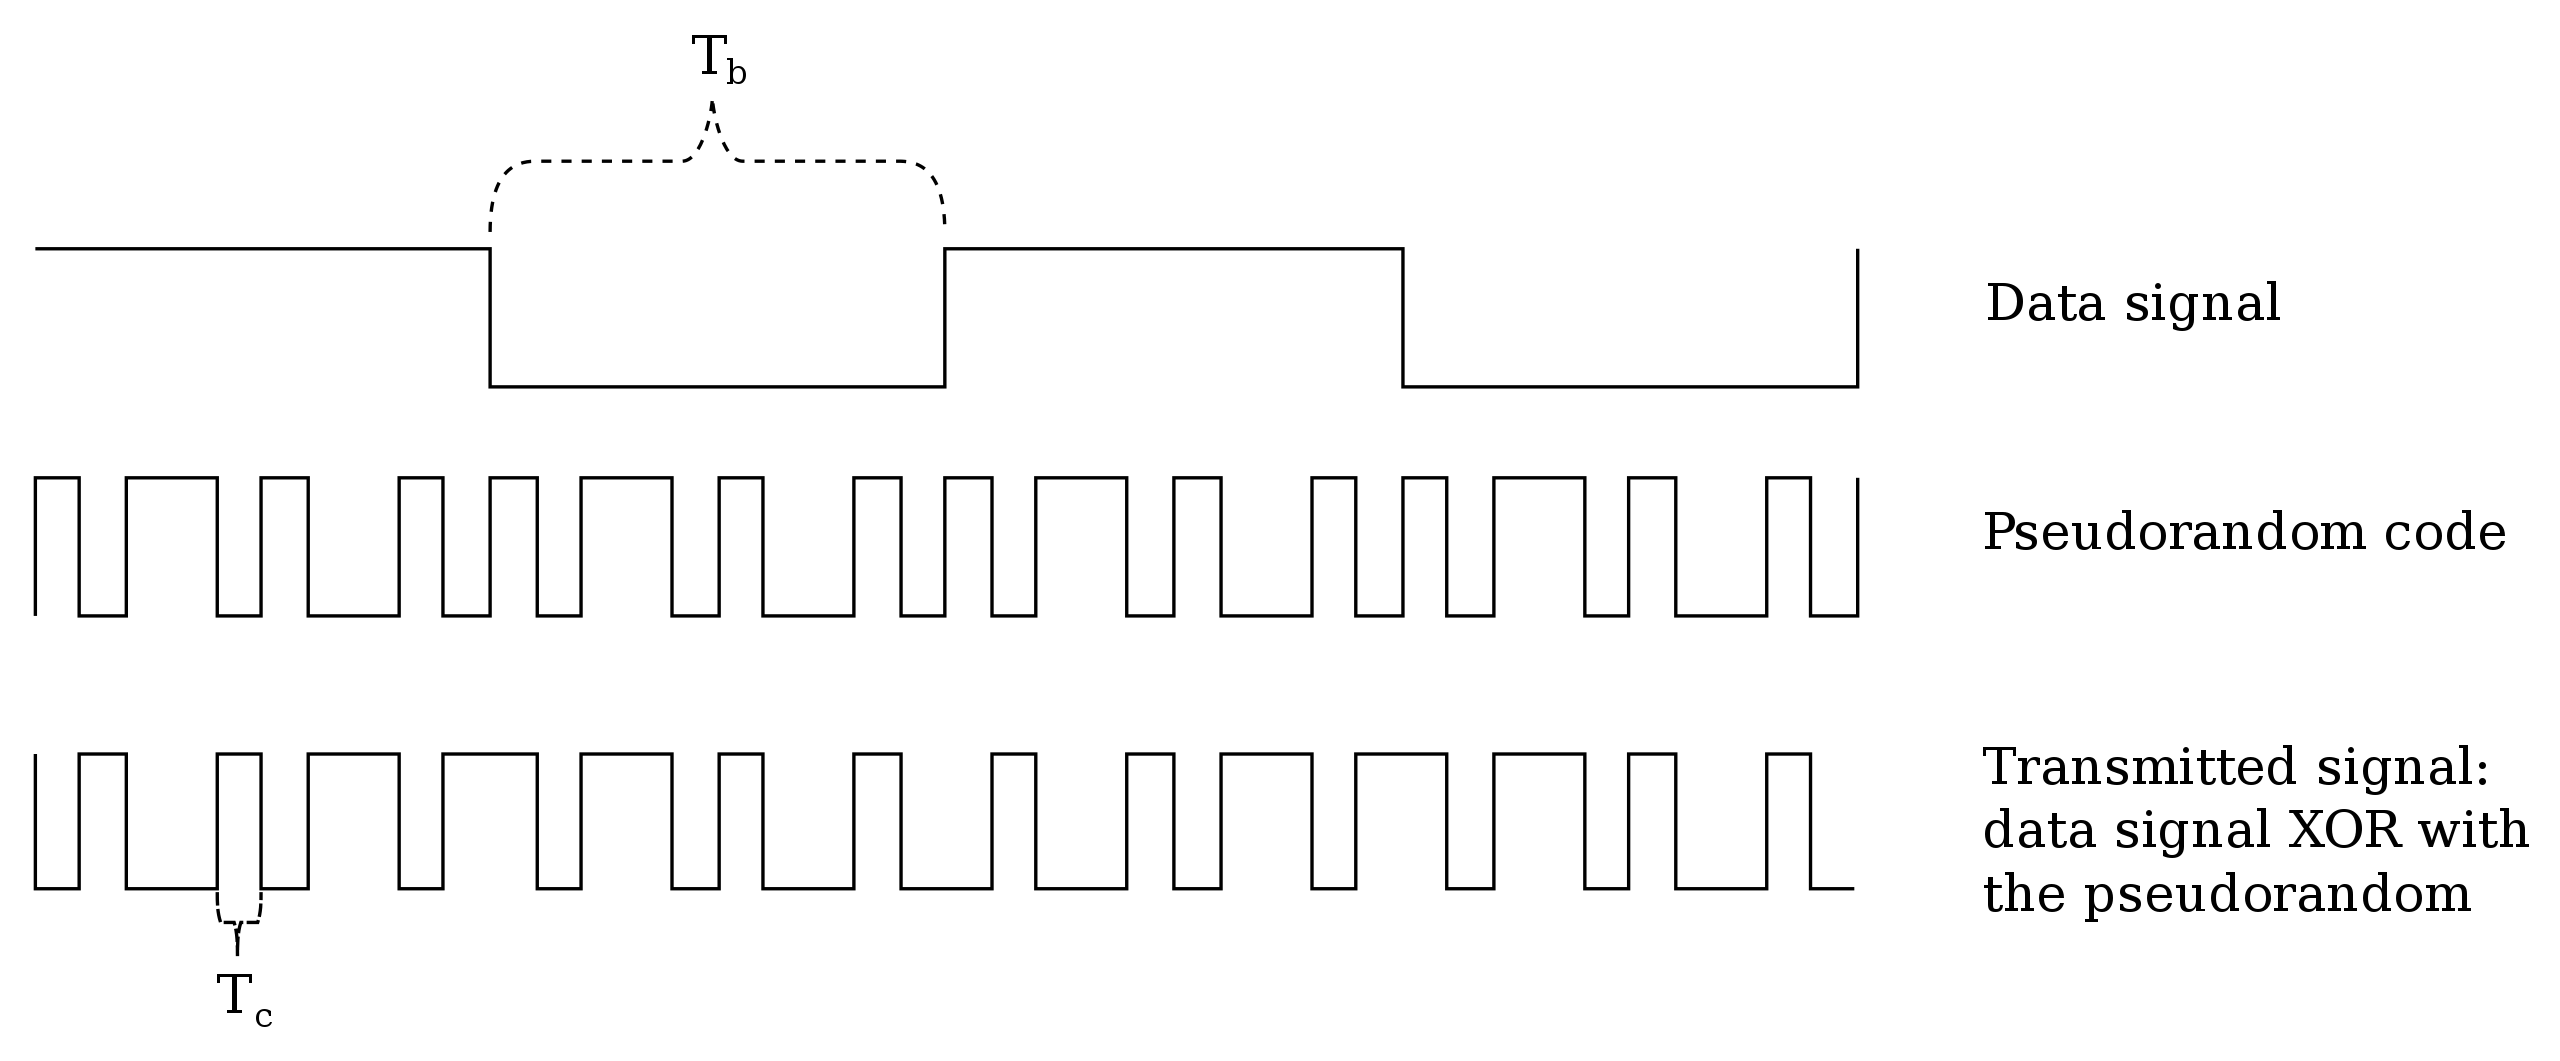
\includegraphics[width=0.8\textwidth]{assets/chap_4/cdma.png}
\end{figure}
\medskip

\noindent
Nếu FDMA chia tần số, TDMA chia thời gian $\rightarrow$ thì CDMA cho phép tất cả mọi người cùng dùng một thời điểm trên cùng một tần số.
\medskip

\noindent
\textbf{Nguyên lý hoạt động:}

\begin{itemize}
    \item \textbf{Truy cập đồng thời} $\rightarrow$ các trạm (host) có thể truy cập môi trường truyền dẫn cùng một lúc và trên cùng một tần số.
    \item \textbf{Mã hóa riêng biệt} $\rightarrow$ mỗi trạm sử dụng một coding schemes (lược đồ mã hóa) khác nhau $\Rightarrow$ tránh bị lẫn lộn tín hiệu của nhau.
    \item \textbf{Orthogonal (tính trực giao)} $\rightarrow$ nghĩa là các mã này hoàn toàn độc lập nhau $\rightarrow$ khi cộng gộp lại, chúng không làm hỏng nhau, và người nhận có thể tách riêng từng mã được (giống kiểu trong phòng ồn ào mà có giọng bạn mình nói thì mình vẫn lọc được).
\end{itemize}
\medskip

\pagebreak

\noindent
\textbf{Cách tạo tín hiệu:}

\noindent
Tín hiệu CDMA được tạo ra bằng phép XOR \textit{(như hình minh họa mô tả)}:

\begin{enumerate}
    \item Data signal $\rightarrow$ tín hiệu dữ liệu gốc (tốc độ chậm).
    \item Pseudorandom code (mã giả ngẫu nhiên) $\rightarrow$ một chuỗi mã ngẫu nhiên giả (tốc độ nhanh) được gán riêng cho người dùng.
    \item Transmitted signal (tín hiệu truyền đi) $\rightarrow$ là kết quả của phép XOR giữa data signal và pseudorandom code.
\end{enumerate}
\medskip

\noindent
$\Rightarrow$ Tín hiệu truyền đi trông giống như một chuỗi ngẫu nhiên (noise) $\rightarrow$ nhưng thật chất nó chứa dữ liệu đã được mã hóa.
\medskip

\noindent
$\rightarrow$ CDMA thường kết hợp với FEC (Forward Error Correction - sửa lỗi tiến) để khôi phục các frame bị lỗi mà không cần gửi lại.
\medskip

\section{Error Control}

\subsection{Failure Causes}

\noindent
Các nguyên nhân gây nên:

\begin{itemize}
    \item \textbf{Signal deformation} (biến dạng tín hiệu) $\rightarrow$ do sự suy hao (attenuation) của môi trường truyền dẫn $\Rightarrow$ tín hiệu càng đi xa thì càng yếu đi $\rightarrow$ nếu quá yếu, máy thu sẽ không phân biệt được đâu là bit 1, đâu là bit 0.
    \item \textbf{Noise} $\rightarrow$ do nhiễu nhiệt hoặc nhiễu điện tử (thermal or electronic noise) $\Rightarrow$ đây là nhiễu sinh ra từ chính các linh kiện điện tử nóng lên, hoặc chuyển động của các electron trong dây dẫn $\rightarrow$ tạo ra các tín hiệu ngẫu nhiên chèn vào dữ liệu thật.
    \item \textbf{Crosstalk (nhiễu xuyên kênh)} $\rightarrow$ do sự can nhiễu từ các kênh lân cận (inference by neighboring channels) $\Rightarrow$ thường do hiện tượng ghép tụ (capacity coupling), đặc biệt tăng mạnh khi tần số tăng cao.
    \item \textbf{Short-time disturbances (nhiễu ngắn hạn)} $\rightarrow$ do các tác động bất ngờ từ bên ngoài; chẳng hạn như bức xạ vũ trụ (cosmic radiation), lớp cách điện bị hỏng hoặc không đủ tốt (defective or insufficient insulation).
\end{itemize}
\medskip

\noindent
\textbf{Lưu ý:} (burst error - lỗi chùm) $\Rightarrow$ lỗi thường không đi lẻ tẻ từng bit (single bit errors) mà thường xảy ra them chùm (burst errors).

$\rightarrow$ Nếu nó đã bị nhiễu $\rightarrow$ sẽ hỏng cả một dây liên tiếp nhiều bit $\rightarrow$ ảnh hưởng đến việc chọn thuật toán sửa lỗi sau này.
\medskip

\noindent
$\Rightarrow$ Data link layer đảm bảo phát hiện và xử lý lỗi truyền trong quá trình gửi/nhận frame.
\medskip

\subsection{Error Detection}

\subsubsection{Checksum}

\noindent
$\rightarrow$ Là một giá trị được tính toán dựa trên nội dung của khối dữ liệu (block of data) bằng một thuật toán định trước (pre-defined algorithm).

$\Rightarrow$ \textbf{Mục đích:} xác minh tính toàn vẹn của dữ liệu (data integrity).
\medskip

\vspace{0.3cm}

\noindent
\textbf{Quy trình:}

\begin{itemize}
    \item \textbf{Sender} $\rightarrow$ tính toán checksum và gắn bó vào cuối mỗi frame.
    \item \textbf{Receiver} $\rightarrow$ khi nhận được frame $\rightarrow$ tính toán lại checksum dựa trên dữ liệu nhận được $\Rightarrow$ nếu kết quả không khớp với checksum $\rightarrow$ frame bị lỗi và sẽ bị loại bỏ (discarded).
\end{itemize}
\medskip

\noindent
\textbf{Possible checksum:}

\begin{itemize}
    \item Parity-check codes $\rightarrow$ kiểm tra tính chẵn lẻ ($\rightarrow$ đơn giản).
    \item Cyclic Redundancy Check (CRC) $\rightarrow$ kiểm tra dư thừa theo chu kỳ ($\rightarrow$ phức tạp và hiệu quả hơn).
\end{itemize}
\medskip

\subsubsection{Hamming Distance}

\noindent
\textbf{Cấu trúc mã (codeword):} một message $n$ bao gồm:

\begin{itemize}
    \item $m$ bit dữ liệu (payload).
    \item $r$ bit checksum.
\end{itemize}
\medskip

\noindent
\textbf{Công thức:} $n = m + r$.
\medskip

\noindent
$\rightarrow$ Trong tổng số $2^n$ chuỗi bit có thể tạo ra $\rightarrow$ chỉ có một số ít là valid codewords (mã hợp lệ) $2^m$.
\medskip

\noindent
\textbf{Hamming distance} $\rightarrow$ là số lượng bit khác nhau nhỏ nhất giữa 2 valid codewords bất kỳ.

$\rightarrow$ Ví dụ: nếu codeword A là \texttt{000} và codeword B là \texttt{011} $\rightarrow$ Hamming distance sẽ là 2 (do khác nhau 2 bit).
\medskip

\noindent
\textbf{Quy tắc để phát hiện lỗi:}

\begin{itemize}
    \item Để phát hiện $k$ lỗi $\rightarrow$ yêu cầu khoảng cách Hamming $d \geq k + 1$. \begin{itemize}
        \item[$\Rightarrow$] Nếu sai $k$ bit $\rightarrow$ nó biến thành một chuỗi vô nghĩa (không trùng với bất kì valid codeword nào) $\rightarrow$ xác định được đây là lỗi.
    \end{itemize}
    \item Để sửa $k$ lỗi $\rightarrow$ yêu cầu khoảng cách Hamming $d \geq 2k + 1$. \begin{itemize}
        \item[$\Rightarrow$] Nếu sai $k$ bit $\rightarrow$ chuỗi bị lỗi vẫn gần với codeword gốc hơn là các codeword khác $\rightarrow$ mình có thể đoán ngược lại để sửa.
    \end{itemize}
\end{itemize}
\medskip

\subsubsection{One-dimensional Parity-check Code}

\begin{center}
\begin{minipage}[c]{0.7\textwidth}
    $\rightarrow$ Nó thêm 1 bit cuối vào dữ liệu $\Rightarrow$ đảm bảo tổng số bit 1 luôn tuân theo quy tắc đã cho.
    \begin{itemize}
        \item \textbf{Cơ chế:} với mỗi khối dữ liệu (chẳng hạn như 1 byte hay 1 kí tự ASCII 7-bit) $\rightarrow$ người ta tính toán và thêm vào 1 bit parity. \begin{itemize}
            \item Protocol defines even parity (chẵn) $\rightarrow$ bit parity được thêm vào sao cho tổng số bit 1 trong cả chuỗi (payload + parity) là một số chẵn.
            \item Protocol defines odd parity (lẻ) $\rightarrow$ bit parity được thêm vào sao cho tổng số bit 1 trong cả chuỗi là một số lẻ.
        \end{itemize}
        \item \textbf{Ví dụ cụ thể:} \textit{(theo hình bên phải)} \begin{itemize}
            \item Với \texttt{0101001} $\rightarrow$ có 3 bit 1 (lẻ) $\rightarrow$ thêm bit parity là 1 để tổng thành 4 (chẵn) $\Rightarrow$ mã cuối cùng là \texttt{0101001 1}.
            \item Với \texttt{1010110} $\rightarrow$ có 4 bit 1 (chẵn) $\rightarrow$ thêm bit parity là 0 để tổng vẫn là 4 (chẵn) $\Rightarrow$ mã cuối cùng là \texttt{1010110 0}.
        \end{itemize}
    \end{itemize}
\end{minipage}
\hfill
\begin{minipage}[c]{0.27\textwidth}
    \centering
    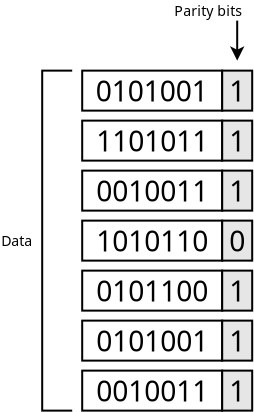
\includegraphics[width=1\textwidth]{assets/chap_4/one-dim.png}
\end{minipage}
\end{center}
\medskip

\noindent
\textbf{What is the Hamming Distance here?}

\begin{itemize}
    \item Cấu trúc: với $m = 7$ bit dữ liệu và $r = 1$ bit parity $\rightarrow$ có codewords dài $n = 8$ bit.
    \item Khoảng cách Hamming $d = 2$ $\Rightarrow$ bất kì 2 valid codewords nào cũng khác nhau ít nhất 2 bit (nếu chỉ thay đổi 1 bit dữ liệu $\rightarrow$ bit parity cũng sẽ buộc phải thay đổi theo $\Rightarrow$ tổng cộng khác 2 bit).
\end{itemize}
\medskip

\noindent
\textbf{Khả năng phát hiện lỗi:} do $d = 2$, theo công thức $d \geq k + 1$ $\rightarrow$ mã này chỉ phát hiện được $k = 1$ lỗi (single-bit error).

$\Rightarrow$ Nếu có 1 bit bị lật $\rightarrow$ tính chẵn lẻ bị sai $\Rightarrow$ phát hiện được error.
\medskip

\noindent
\textbf{Limitation:} nếu có 2 bit cùng bị lật ($1 \rightarrow 0$ và $0 \rightarrow 1$) $\Rightarrow$ không phát hiện được lỗi.
\medskip

\noindent
$\Rightarrow$ Phương pháp này đơn giản $\rightarrow$ phù hợp cho các khối dữ liệu ngắn (short blocks of data); chẳng hạn như 7-bit ASCII characters.

$\rightarrow$ Không đáng tin cậy nếu đường truyền quá nhiễu (gây nhiều lỗi bit cùng lúc).
\medskip

\subsubsection{Two-dimensional Parity-check Code}

\begin{center}
\begin{minipage}[c]{0.7\textwidth}
    $\rightarrow$ 2D parity-check code sẽ scan dữ liệu theo cả hàng lẫn cột, khác với 1D chỉ scan theo hàng $\Rightarrow$ tạo thành matrix để bắt lỗi tốt hơn.
    \begin{itemize}
        \item \textbf{Cơ chế:} dữ liệu được sắp xếp thành một bảng (matrix). \begin{itemize}
            \item Rows $\rightarrow$ với mỗi byte dữ liệu $\rightarrow$ mình tính 1 bit parity gắn vào cuối (giống y như phương pháp 1D).
            \item Columns $\rightarrow$ tính cho tất cả các bit ở cột 1, 2, ... $\rightarrow$ kết quả tạo thành 1 byte đặc biệt nằm dưới cùng $\Rightarrow$ gọi là parity byte.
        \end{itemize}
        \item \textbf{Ví dụ cụ thể:} \textit{(theo hình bên phải)} \begin{itemize}
            \item Tính hàng ngang \textit{(như 1D ở trên)}.
            \item Tính hàng dọc: tương tự như cách tính ở hàng ngang; ví dụ như cột đầu tiên ở mỗi hàng là \texttt{0}, \texttt{1}, \texttt{0}, \texttt{1}, \texttt{0}, \texttt{0}, \texttt{0} $\rightarrow$ tổng bit 1 là chẵn $\rightarrow$ bit parity cột là \texttt{0}.
        \end{itemize}
    \end{itemize}
\end{minipage}
\hfill
\begin{minipage}[c]{0.27\textwidth}
    \centering
    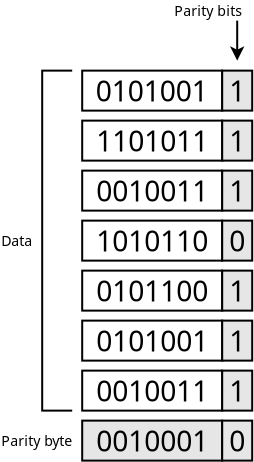
\includegraphics[width=1\textwidth]{assets/chap_4/two-dim.png}
\end{minipage}
\end{center}
\medskip

\noindent
Ở loại 1D, nếu 2 bit trong cùng 1 hàng bị lỗi $\rightarrow$ tổng số bit 1 vẫn không đổi (chẵn/lẻ) $\Rightarrow$ không phát hiện được lỗi.

$\Rightarrow$ Đối với 2D, nếu 2 bit trong cùng 1 hàng bị sai $\rightarrow$ parity hàng ngang không báo lỗi $\Rightarrow$ nhưng parity hàng dọc của 2 cột chứa 2 bit sai đó sẽ bị lệch $\rightarrow$ phát hiện được lỗi.
\medskip

\vspace{0.1cm}

\textbf{$\rightarrow$ Phạm vi phát hiện:} tất cả các lỗi 1 bit, 2 bit, và 3 bit, và hầu hết các lỗi 4 bit đều được phát hiện.
\medskip

\subsubsection{Cyclic Redundancy Check (CRC)}

\noindent
$\rightarrow$ Là phương pháp phát hiện lỗi mạnh mẽ hơn nhiều so với parity check $\rightarrow$ được sử dụng rộng rãi (như trong Ethernet, Wifi).
\medskip

\begin{itemize}
    \item Mọi chuỗi bit đều có thể được viết dưới dạng một đa thức với hệ số là 0 hoặc 1.
    \item Một frame có $k$ bit được xem như một đa thức bậc $k-1$.
\end{itemize}
\medskip

\noindent
\textbf{Ví dụ:} chuỗi \texttt{10011010} tương ứng với đa thức:

\[
\begin{aligned}
M(x) &= 1x^7 + 0x^6 + 0x^5 + 1x^4 + 1x^3 + 0x^2 + 1x + 0 \\
    &= x^7 + x^4 + x^3 + x
\end{aligned}
\]
\medskip

\subsubsection{CRC Generator Polynomial}

\noindent
Để sender và receiver hiểu nhau $\rightarrow$ phải thống nhất trước một công thức toán học cụ thể $\rightarrow$ là đa thức sinh $C(x)$ (generator polynomial).
\medskip

\noindent
\textbf{Cách biểu diễn:} máy tính không hiểu $x^5$ hoặc $x^2$ $\rightarrow$ đa thức được chuyển đổi thành chuỗi bit dựa trên các hệ số.

\begin{itemize}
    \item Nếu có $x^n$ $\rightarrow$ bit tại vị trí $n$ là 1.
    \item Nếu thiếu $x^n$ $\rightarrow$ bit tại vị trí $n$ là 0.
\end{itemize}
\medskip

\noindent
\textbf{Ví dụ:} đa thức $C(x) = x^3 + x^2 + x^0 = 1 \cdot x^3 + 1 \cdot x^2 + 0 \cdot x^1 + 1 \cdot x^0$.

$\rightarrow$ Chuỗi bit tương ứng là \texttt{1101}.
\medskip

\noindent
\textbf{Bậc của đa thức (degree - $k$):}

\begin{itemize}
    \item Bậc $k$ là số mũ cao nhất trong đa thức $\rightarrow$ số lượng bit của chuỗi nhị phân luôn nhiều hơn bậc $k$ một đơn vị (độ dài chuỗi là $k+1$).
    \item \textbf{Ví dụ:} \texttt{1101} có 4 bit $\rightarrow$ bậc $k = 3$.
\end{itemize}
\medskip

\noindent
$\rightarrow$ Nếu dùng đa thức bậc $k$ $\rightarrow$ phần dư (checksum) tạo ra sẽ luôn có $k$ bit (được thêm vào sau dữ liệu).
\medskip

\noindent
\textbf{Representation:} với đa thức sinh bậc $k$ $\rightarrow$ người ta thường lấy $k-1$ để biểu diễn; ví dụ, đa thức trên (\texttt{1101}) người ta sẽ lấy $k-1$ (tương ứng \texttt{101}) để biểu diễn $\rightarrow$ thành \texttt{0x05}.
\medskip

\subsubsection{Selection of common Generator Polynomials}

\begin{table}[h]
    \renewcommand{\arraystretch}{1.2}
    \begin{tabular*}{\linewidth}{@{\extracolsep{\fill}}llll}
        \hline
        \textbf{Tên chuẩn} & \textbf{Đa thức} & \textbf{Chuỗi bit (Hex/Bin)} & \textbf{Ứng dụng} \\
        \hline
        CRC-5 & $x^5 + x^2 + x^0$ & \texttt{0x05} & USB \\
        CRC-8 & $x^8 + x^7 + x^5 + x^2 + x^1 + x^0$ & \texttt{0xA7} & Bluetooth \\
        CRC-16-CCITT & $x^{16} + x^{12} + x^5 + x^0$ & \texttt{0x1021} & HDLC \\
        CRC-32 & $x^{32} + ... + x^0$ & \texttt{0x04C11DBB7} & Ethernet \\
        \hline
    \end{tabular*}
\end{table}
\medskip

\subsubsection{CRC Example}

\noindent
(Tự đọc)
\medskip

\subsubsection{Properties of CRCs}

\noindent
\textbf{Single bit errors (phát hiện tất cả các lỗi đơn):}

\begin{itemize}
    \item \textbf{Điều kiện:} nếu đa thức sinh $G(x)$ có nhiều hơn một số hạng (nghĩa là có ít nhất 2 bit 1; chẳng hạn như $x^5 + x^0$), và hệ số của $x^0$ là 1 (bit cuối là 1 chứ không phải là 0).
    \item[$\Rightarrow$] Bất kì lỗi nào chỉ sai 1 bit duy nhất đều bắt được.
\end{itemize}
\medskip

\noindent
\textbf{Double bit errors (phát hiện tất cả các lỗi kép):}

\begin{itemize}
    \item \textbf{Điều kiện:} đa thức sinh không chia hết cho $x^k + 1$ $\forall k$ nhỏ hơn độ dài của khung tin tối đa.
    \item[$\Rightarrow$] Nếu có 2 bit bị sai nằm cách nhau một khoảng (trong giới hạn cho phép) $\rightarrow$ CRC vẫn phát hiện được.
\end{itemize}
\medskip

\noindent
\textbf{Odd number of errors (phát hiện bất kì số lượng lỗi lẻ nào):}

\begin{itemize}
    \item \textbf{Điều kiện:} nếu đa thức sinh $G(x)$ có chứa thừa số $(x+1)$.
    \item[$\Rightarrow$] Dù có sai 3 bit, 5 bit, ... (miễn là số lượng bit sai là số lẻ) $\rightarrow$ CRC đều phát hiện được.
\end{itemize}
\medskip

\noindent
\underline{Self-note:} đây là lý do tại sao nhiều chuẩn CRC (như CRC-16 hay CRC-32) đều có thừa số $(x+1)$ trong đa thức sinh của chúng.
\medskip

\vspace{0.2cm}

\noindent
\textbf{Burst error (phát hiện lỗi chùm):}
\medskip

\noindent
$\rightarrow$ Nhiễu làm hỏng cả một dây liên tiếp các bit.
\medskip

\noindent
Gọi $r$ là bậc của đa thức sinh (chẳng hạn như CRC-16 thì $r = 16$).

\begin{itemize}
    \item \textbf{Chiều dài chùm lỗi là $L \leq r$} $\rightarrow$ CRC phát hiện được tất cả lỗi; ví dụ như dùng CRC-16, nếu bị nhiễu nguyên một đoạn 16 bit liên tiếp hoặc ít hơn thì nó vẫn bắt lỗi được hết.
    \item \textbf{Chiều dài chùm lỗi là $L = r+1$} $\rightarrow$ xác suất phát hiện là $1-2^{-(r-1)}$ \textit{(để cho biết chứ không cần nhớ)}; như CRC-16 có tỉ lệ phát hiện lỗi lên đến $\approx$99.997\%.
    \item \textbf{Chiều dài chùm lỗi là $L > r+1$} $\rightarrow$ xác suất phát hiện là $1-2^{-r}$ \textit{(để cho biết chứ không cần nhớ)}; như CRC-16 có tỉ lệ phát hiện lỗi lên đến $\approx$99.998\% với độ dài lên đến $\geq 18$.
\end{itemize}
\medskip

\noindent
$\rightarrow$ CRC có thể được tính toán thông qua kỹ thuật dịch bit (shift register).
\medskip

\pagebreak

\subsection{Error Correction}

\subsubsection{Forward Error Correction (FEC)}

\begin{itemize}
    \item \textbf{Cách cũ:} error detection + retransmission $\rightarrow$ thấy lỗi, báo hỏng, rồi xin gửi lại $\Rightarrow$ tốn thời gian, và độ trễ cao.
    \item \textbf{Với FEC:} khi thấy lỗi $\rightarrow$ dùng dữ liệu dư thừa (redundant information) để tính toán và khôi phục lại bit gốc.
\end{itemize}
\medskip

\noindent
\textbf{Điều kiện (dựa theo quy tắc Hamming):}
\medskip

\noindent
Codewords phải theo khoảng cách Hamming $d \geq 2k + 1$.

\textbf{Trong đó:} $k$ $\rightarrow$ số lượng bit lỗi tối đa mà mình muốn sửa được.
\medskip

\noindent
$\Rightarrow$ Nếu muốn sửa 1 bit lỗi ($k=1$) $\rightarrow$ khoảng cách giữa các valid codewords phải là: $2 \cdot (1) + 1 = 3$.
\medskip

\noindent
\textbf{Nguyên lý hoạt động:} người gửi sẽ chèn thêm rất nhiều redundancy information vào dữ liệu.

\begin{itemize}
    \item Dữ liệu gốc ($m$ bits) được mã hóa thành chuỗi dài hơn ($n$ bits); tỉ lệ mã hóa (code rate) $R = m/n$ nhỏ hơn 1.
    \item \textbf{Ví dụ:} muốn gửi 1 bit dữ liệu $\rightarrow$ có khi phải gửi kèm 2 bit sửa lỗi $\Rightarrow$ gửi tổng cộng 3 bit $\rightarrow$ tốn băng thông nhưng an toàn.
\end{itemize}
\medskip

\noindent
\textbf{Khi nào dùng FEC?}

\begin{itemize}
    \item High delay (độ trễ cao) $\rightarrow$ chẳng hạn như truyền vệ tin với khoảng cách xa $\rightarrow$ nếu chờ gửi lại thì tốn rất nhiều thời gian $\Rightarrow$ tự sửa lỗi sẽ nhanh hơn.
    \item High error rates (tỉ lệ lỗi cao) $\rightarrow$ như mạng không dây $\rightarrow$ nếu cứ một xíu là xin gửi lại thì sẽ gây ngẽn mạng.
    \item Không có kênh phản hồi (no backward channel) $\rightarrow$ như truyền hình hay đài phát thanh, người nghe chỉ nhận chứ không feedback lại cho nhà đài liền được.
\end{itemize}
\medskip

\noindent
\textbf{Nhược điểm:}

\begin{itemize}
    \item Overhead (tốn băng thông) $\rightarrow$ phải gửi nhiều bit dư thừa hơn mức cần thiết.
    \item Phức tạp $\rightarrow$ thuật toán giải mã (decoding algorithm) để tìm và sửa lỗi thường phức tạp hơn nhiều so với việc chỉ kiểm tra (detection).
\end{itemize}
\medskip

\subsubsection{Simple Example of Error Correction}

\noindent
Giả sử một code chỉ có 4 valid codewords:

\begin{itemize}
    \item $w_1 = $ \texttt{00000 00000}.
    \item $w_2 = $ \texttt{00000 11111}.
    \item $w_3 = $ \texttt{11111 00000}.
    \item $w_4 = $ \texttt{11111 11111}.
\end{itemize}
\medskip

\noindent
Ta có:

\begin{itemize}
    \item $w_1 \not= w_2$ $\rightarrow$ 5 bit cuối.
    \item $w_1 \not= w_3$ $\rightarrow$ 5 bit đầu.
    \item $w_1 \not= w_4$ $\rightarrow$ tất cả 10 bit.
\end{itemize}
\medskip

\noindent
$\Rightarrow$ Khoảng cách nhỏ nhất là 5 $\rightarrow$ $d = 5$.

\begin{itemize}
    \item \textbf{Để detection:} $d \geq k + 1$ $\rightarrow$ $k \leq 4$ $\Rightarrow$ có thể phát hiện tối đa 4 bit lỗi.
    \item \textbf{Để correction:} $d \geq 2k + 1$ $\rightarrow$ $k \leq 2$ $\Rightarrow$ có thể sửa tối đa 2 bit lỗi.
\end{itemize}
\medskip

\noindent
\textbf{Ví dụ:}

\begin{itemize}
    \item Nếu máy nhận được \texttt{00000 00111} $\rightarrow$ nó sẽ đem so với $w_1$ (sai 3 bit) và $w_2$ (sai 2 bit) $\Rightarrow$ chọn $w_2$ làm codeword gốc $\rightarrow$ sửa lại thành \texttt{00000 11111}.
    \item[$\Rightarrow$] Tuy nhiên, nếu sender gửi đi \texttt{00000 00000} nhưng bị nhiễu thành \texttt{00000 00111} $\rightarrow$ máy thấy gần với $w_2$ hơn $\Rightarrow$ sửa thành \texttt{00000 11111} $\rightarrow$ sai hoàn toàn với dữ liệu gốc.
\end{itemize}
\medskip

\noindent
$\rightarrow$ Với $d = 5$: hệ thống chỉ đảm bảo sửa đúng nếu lỗi $\leq 2$ bit $\Rightarrow$ nếu lỗi 3 bit trở lên, hệ thống sẽ bị lầm và sửa sai thành frame khác.
\medskip

\pagebreak
